\documentclass[10pt,spanish,xcolor={svgnames}]{beamer}
%%documentclass[notes,spanish,10pt]{beamer}       % print frame + notes

% TILDES Y DEMÁS EN ESPAÑOL
\usepackage[spanish]{babel}
\usepackage{fontspec} 
\setmainfont{Fira Sans Ultralight} 
\setsansfont{Fira Sans Ultralight} 
\setmonofont{Fira Mono Regular} 
\usetheme[numbering=fraction, progressbar=head]{metropolis}
\usepackage{appendixnumberbeamer}
%%	NUMEROS COMO FRACCIONS 4/20 Y BARRA DE PROGRESO EN CADA DIAPOSITIVA (TOO MUCH?)
%\setsansfont[BoldFont={Fira Sans SemiBold}]{Fira Sans Book} %TEXTO QUE SE LEE MEJOR PARA UNA SALA GRANDE Y PROYECTOR CON POCA POTENCIA

\usepackage{booktabs}
\usepackage[scale=2]{ccicons}

\usepackage{pgfplots}
\usepgfplotslibrary{dateplot}
\usepackage{xspace}
\newcommand{\themename}{\textbf{\textsc{metropolis}}\xspace}
% \setbeamertemplate{footline}[frame number] % PARA PONER EL NUMERO DE PAGINA EN FRACCIÓN: 7/20

% Comando para poder añadir la fuente en mis figuras
\newcommand{\source}[1]{{\textbf{Fuente}: {#1}} }

\usepackage{hyperref} % LINKS

%PARA LA TABLAS
 \usepackage{booktabs}
 \usepackage{newtxtext, newtxmath}
 \usepackage{threeparttable}
 \usepackage{graphicx}
 \usepackage[binary-units=true]{siunitx}
\renewcommand{\tablename}{Tabla} %para nombrar Tablas a las tablas.



\usepackage{pgfpages} %PARA LAS NOTAS
\setbeameroption{show notes}                        
\setbeameroption{show notes on second screen=right} %% en terminal, $: pdfpc main.pdf --notes=right
%https://bugs.kde.org/show_bug.cgi?id=152585


\setbeamertemplate{note page}{\pagecolor{yellow!5}\insertnote}% MUY IMPORTANTE, ASÍ MUESTRA TAN SOLO UNA NOTA EN  BLANCO EN VEZ DE MOSTRAR UNA DIAPO DE NOTA ESTRUCTURADA (UNA PARTE ES LA NOTA EN SI, OTRA LA SIGUIENTE DIAPO Y OTRA EL ARBOL (SECCION->SUBSECCION->TITLE _RAME) Y NO QUEREMOS ESO.
%\usepackage{palatino}  % SI DESCOMENTO ESTO SE ME JOROBAN TODAS LAS FUENTES DE LAS DIAPOS. NO TOCAR LA FUENTE DE LAS NOTAS.



%para que funcionen bien las notas, pero mandarlo a tomar por saco, sin ello no se notaba diferencia
%\makeatletter\def\beamer@framenotesbegin{%atbeginningofslide
%\usebeamercolor[fg]{normal text}\gdef\beamer@noteitems{}%
%\gdef\beamer@notes{}%
%}\makeatother


\usepackage{dirtytalk} % PARA CITAR, CITAS, QUOTES.

%TODOs notas:
%\usepackage[colorinlistoftodos,prependcaption,textsize=small]{todonotes} %% PARA QUE NO APAREZCAN [disable]


%\usepackage{xcolor} % CAMBIAR TEXTO DE COLOR (PARA LAS NOTAS)
\usepackage{wrapfig} % FIGURAS  A UN LADO, CON TEXTO AL OTRO.

\usepackage[export]{adjustbox} %PONER A LA IZQUIERDA LAS FIGURAS, NECESARIO PARA USAR \left y \right. 	eg.\includegraphics..[\textwidth,\left]..



%%%%%%%%%%%%%%%%%%%%%%%%%%%%%%%%%%%%%%%%%%%%%%%%%%%%
%%%%%%%%%%%%%%%%%%%%%%%%%%%%%%%%%%%%%%%%%%%%%%%%%%%%
%%%%%%%%%%%%%%%%%%%%%%%%%%%%%%%%%%%%%%%%%%%%%%%%%%%%
%%%%%%%%%%%%%%%%%%%%%%%%%%%%%%%%%%%%%%%%%%%%%%%%%%%%
%%%%%%%%%%%%%%%%%%%%%%%%%%%%%%%%%%%%%%%%%%%%%%%%%%%%
%%%%%%%%%%%%%%%%%%%%%%%%%%%%%%%%%%%%%%%%%%%%%%%%%%%%
%%%%%%%%%%%%%%%%%%%%%%%%%%%%%%%%%%%%%%%%%%%%%%%%%%%%
%%%%%%%%%%%%%%%%%%%%%%%%%%%%%%%%%%%%%%%%%%%%%%%%%%%%
%%%%%%%%%%%%%%%%%%%%%%%%%%%%%%%%%%%%%%%%%%%%%%%%%%%%
%%%%%%%%%%%%%%%%%%%%%%%%%%%%%%%%%%%%%%%%%%%%%%%%%%%%
%%%%%%%%%%%%%%%%%%%%%%%%%%%%%%%%%%%%%%%%%%%%%%%%%%%%
%%%%%%%%%%%%%%%%%%%%%%%%%%%%%%%%%%%%%%%%%%%%%%%%
\usepackage{framed}
\usepackage{ifxetex,ifluatex}
\usepackage{etoolbox} 
% conditional for xetex or luatex
\newif\ifxetexorluatex
\ifxetex
  \xetexorluatextrue
\else
  \ifluatex
    \xetexorluatextrue
  \else
    \xetexorluatexfalse
  \fi
\fi
%
\ifxetexorluatex%
  \usepackage{fontspec}
  \setmainfont{Fira Sans Ultralight} % or use \setmainfont to choose any font on your system
  \newfontfamily\quotefont[Ligatures=TeX]{Fira Sans Ultralight} % selects Libertine as the quote font
\fi

\newcommand*\quotesize{60} % if quote size changes, need a way to make shifts relative
% Make commands for the quotes
\newcommand*{\openquote}
   {\tikz[remember picture,overlay,xshift=-4ex,yshift=-2.5ex]
   \node (OQ) {\quotefont\fontsize{\quotesize}{\quotesize}\selectfont``};\kern0pt}

\newcommand*{\closequote}[1]
  {\tikz[remember picture,overlay,xshift=4ex,yshift={#1}]
   \node (CQ) {\quotefont\fontsize{\quotesize}{\quotesize}\selectfont''};}

% select a colour for the shading
\colorlet{shadecolor}{Azure}

\newcommand*\shadedauthorformat{\emph} % define format for the author argument

% Now a command to allow left, right and centre alignment of the author
\newcommand*\authoralign[1]{%
  \if#1l
    \def\authorfill{}\def\quotefill{\hfill}
  \else
    \if#1r
      \def\authorfill{\hfill}\def\quotefill{}
    \else
      \if#1c
        \gdef\authorfill{\hfill}\def\quotefill{\hfill}
      \else\typeout{Invalid option}
      \fi
    \fi
  \fi}
% wrap everything in its own environment which takes one argument (author) and one optional argument
% specifying the alignment [l, r or c]
%
\newenvironment{shadequote}[2][l]%
{\authoralign{#1}
\ifblank{#2}
   {\def\shadequoteauthor{}\def\yshift{-2ex}\def\quotefill{\hfill}}
   {\def\shadequoteauthor{\par\authorfill\shadedauthorformat{#2}}\def\yshift{2ex}}
\begin{snugshade}\begin{quote}\openquote}
{\shadequoteauthor\quotefill\closequote{\yshift}\end{quote}\end{snugshade}}

%%%%%%%%%%%%%%%%%%%%%%%%%%%%%%%%%%%%%%%%%%%%%%%%%%%%
%%%%%%%%%%%%%%%%%%%%%%%%%%%%%%%%%%%%%%%%%%%%%%%%%%%%
%%%%%%%%%%%%%%%%%%%%%%%%%%%%%%%%%%%%%%%%%%%%%%%%%%%%
%%%%%%%%%%%%%%%%%%%%%%%%%%%%%%%%%%%%%%%%%%%%%%%%%%%%
%%%%%%%%%%%%%%%%%%%%%%%%%%%%%%%%%%%%%%%%%%%%%%%%%%%%
%%%%%%%%%%%%%%%%%%%%%%%%%%%%%%%%%%%%%%%%%%%%%%%%%%%%
%%%%%%%%%%%%%%%%%%%%%%%%%%%%%%%%%%%%%%%%%%%%%%%%%%%%
%%%%%%%%%%%%%%%%%%%%%%%%%%%%%%%%%%%%%%%%%%%%%%%%%%%%
%%%%%%%%%%%%%%%%%%%%%%%%%%%%%%%%%%%%%%%%%%%%%%%%%%%%
%%%%%%%%%%%%%%%%%%%%%%%%%%%%%%%%%%%%%%%%%%%%%%%%%%%%
%%%%%%%%%%%%%%%%%%%%%%%%%%%%%%%%%%%%%%%%%%%%%%%%%%%%
%%%%%%%%%%%%%%%%%%%%%%%%%%%%%%%%%%%%%%%%%%%%%%%%%%%%
%%%%%%%%%%%%%%%%%%%%%%%%%%%%%%%%%%%%%%%%%%%%%%%%%%%%


%%%%%%%%%%%%%%%%%%%%%%%%%%%%%%%%%%%%%%%%%%%%%%%%%%%%%%%%%%%%%%%%%%%%%%%%%%%%%%%%
%%%%%%%%%%%%%%%%%%%%%%%%%%%%%%%%%%%%%%%%%%%%%%%%%%%%%%%%%%%%%%%%%%%%%%%%%%%%%%%%
%%%%%%%%%%%%%%%%%%%%%%%%%%%%%%%%%%%%%%%%%%%%%%%%%%%%%%%%%%%%%%%%%%%%%%%%%%%%%%%%
% DATOS DE LA PORTADA Y DEMÁS
%%%%%%%%%%%%%%%%%%%%%%%%%%%%%%%%%%%%%%%%%%%%%%%%%%%%%%%%%%%%%%%%%%%%%%%%%%%%%%%%
%%%%%%%%%%%%%%%%%%%%%%%%%%%%%%%%%%%%%%%%%%%%%%%%%%%%%%%%%%%%%%%%%%%%%%%%%%%%%%%%
%%%%%%%%%%%%%%%%%%%%%%%%%%%%%%%%%%%%%%%%%%%%%%%%%%%%%%%%%%%%%%%%%%%%%%%%%%%%%%%%


\title{Estudio de técnicas de Ingeniería de Tráfico basadas en SDN}
\subtitle{Study of SDN Traffic Engineering Techniques}

%\author{Betegon Garcia, Miguel}
%\institute{Center for modern beamer themes}
\author[M. Betegón]{ Betegón García, Miguel\inst{1} \\ {\ttfamily miguel.betegon@alumnos.unican.es}} 

\institute[UC] % (optional)
{
	\inst{1}%
	Grado en Ingeniería de Tecnologías de Telecomunicación
}
%\date{\today}
\date{Julio, 2018}

\titlegraphic{
	
	
\includegraphics[width=3.5em]{figuras/uc.png}\hfill
	
\includegraphics[width=5em]{figuras/uccc_no_letras.png}\hfill
	
\includegraphics[width=3.2em]{figuras/git.png}
}

\setbeamertemplate{title page}{
	\begin{minipage}[b][\paperheight]{\textwidth}
		\vfill%
		\ifx\inserttitle\@empty\else\usebeamertemplate*{title}\fi
		\ifx\insertsubtitle\@empty\else\usebeamertemplate*{subtitle}\fi
		\usebeamertemplate*{title separator}
		\ifx\beamer@shortauthor\@empty\else\usebeamertemplate*{author}\fi
		\ifx\insertdate\@empty\else\usebeamertemplate*{date}\fi
		\ifx\insertinstitute\@empty\else\usebeamertemplate*{institute}\fi
		\vfill
		\ifx\inserttitlegraphic\@empty\else\inserttitlegraphic\fi
		\vspace*{1cm}
	\end{minipage}
}

%	\titlegraphic{\vspace{-1.6em}\includegraphics[height=1.5cm]{logo.pdf}}
\pgfplotsset{width=10cm,compat=1.9}
\usepackage{pgfplotstable}

\newcommand{\nologo}{\setbeamertemplate{logo}{}} % CREAMOS \nologo que es un logo vacio, para poder quitar el logo en las diapos que tengan figuras que ocupen bastante.


%% ---- COMIENZA EL DOCUMENTO ----
%%%%%%%%%%%%%%%%%%%%%%%%%%%%%%%%%%%%%%%%%%%%%%%%%%%%%%%%%%%%%%%%%%%%%%%%%%%%%%%%%%%%%%%%%%%%%%%%%%%%%%%%%%%%%%%%%%%%%%%%%%%%%%%%%%%%%%%%%%%%%%%%%%%%%%%%%%%%%%%%%%%%%%%%%%%%%%%%%%%%%%%%%%%%%%%%%%%%%%%%%%%%%%%%%%%%%%%%%%%%%%%%%%%%%%%%%%%%%%%%%%%%%%%%%%%%%%%%%%%%%%%%%%%%%%%%%%%%%%%%%%%%%%%%%%%%%%%%%%%%%%%%%%%%%%%%%%%%%%%%%%%%%%%%%%%%%%%%%%%%%%%%%%%%%%%%%%%%%%%%%%%%%%%%%%%%%%%%%%%%%%%%%%%%%%%%%%%%%%%%%%%%%%%%%%%%%%%%%%%%%%%%%%%%%%%%%%%%%%%%%%%%%%%%%%%%%%%%%%%%%%%%%%%%%%%%%%%%%%%%%%%%%%%%%%%%%%%%%%%%%%%%%%%%%%%%%%%%%%%%%%%%%%%%%%%%%%%%%%%%%%%%%%%%%%%%%%%%%%%%%%%%%%%%%%%%%%%%%%%%%%%%%%%%%%%%%%%%%%%%%%%%%%%%%%%%%%%%%%%%%%%%%%%%%%%%%%%%%%%%%%%%%%%%%%%%%%%%%%%%%%%%%%%%%%%%%%%%%%%%%%%%%%%%%%%%%%%%%%%%%%%%%%%%%%%%%%%%%%%%%%%%%%%%%%%%%%%%%%%%%%%%%%%%%%%%%%%%%%%%%%%%%%%%%%%%%%%%%%%%%%%%%%%%%%%%%%%%%%%%%%%%%%
\begin{document}

\begin{frame}
  \titlepage
		\note[item]{\textcolor{red}{EN LA TERMINAL, \$: pdfpc main.pdf - -notes=right}}
% 		\note[item]{\textcolor{red}{https://bugs.kde.org/show\_bug.cgi?id=152585}}
% 		\note[item]{\textcolor{red}{ESTOY COMPILANDO DESDE OVERLEAF CON XUALATEX. CON XELATEX PUEDE FUNCIONAR CREO, PERO CON PDFlatex no. PDFlatex no entiende la fuente (fira) y utiliza las suyas}}
% 			\note[item]{\textcolor{red}{CUIDADO, SE ME PONE EL TEXTO DE COLOR BLANCO Y NO SE VE, ES CULPA DE USAR NOTAS (PFGPAGES) Y XELATEX}}
%             \note[item]{\textcolor{red}{SI USO TODOs SE JOROBA LA FUENTE Y DA ERRORES. POR ESO HE PUESTO EL TEXTO QUE NO ES DE NOTAS SINO DE COSAS PARA CAMBIAR DE LAS DIAPOSITIVAS EN ROJO}}
%             \note[item]{\textcolor{red}{ECHAR UN OJO A LA PORTADA, POR SI NO PRESENTARÁ EN JUNIO (Pone Junio, 2018)}}
\end{frame}


%SI NO ME GUSTA COMO PONGO LA PORTADA (begin frame... titlepage...) la puedo poner como la tenía antes, \maketitle sólo, sin begin frame ni nada. Está puesto con Begin frame porque así puedo añadir notas en esa diapo.
%\maketitle

% DEFINO EL LOGO AQUÍ PARA QUE NO ME APAREZCA EN EN LA DIAPOSITIVA DE PORTADA (EN LA PORTADA LO PONGO A MANO PARA QUE ESTÉ ALINEADO CON EL RESTO DE LOGOS).
\logo{

\includegraphics[width=1.1cm,keepaspectratio]{figuras/git.png}
}


\begin{frame}{Índice}
	\setbeamertemplate{section in toc}[sections numbered]
	\tableofcontents[hideallsubsections]
    \note{\LARGE \vfill
		\begin{center}
			\begin{enumerate}
				\item Comenzaré con ... le seguiran los conceptos teóricos en los que se basa el proyecto, después  se comentará la parte técnica antes de pasar a la implementación y por último acabaré con las conclusiones y lineas futuras.
				\vfill
			\end{enumerate}
		\end{center}}
\end{frame}
%%%%%%%%%%%%%%%%%%%%%%%%%%%%%%%%%%%%%%%%%%%%%%%%%%%%%%%%%
%%%%%%%%%%%%%%%%%%
%% INTRODUCCIÓN %%
%%%%%%%%%%%%%%%%%%
\section{Introducción}


\begin{frame}{Motivación y objetivos I}
\vspace{-2em}
Las redes definidas por software (SDN) surgen a principios de 2010 \alert{por necesidad}:
\begin{itemize}
	\item La mayoría de las redes tradicionales fueron diseñadas como aplicaciones cliente-servidor que se ejecutan en una infraestructura no virtualizada.
\end{itemize}

SDN se ha establecido como un producto conocido.

Es una realidad que muchas de las empresas y proveedores de servicios de todo el mundo ya han adoptado.


\note{\large \vfill
	\begin{center}
	\begin{enumerate}
		\item NO son la solución a un problema sin resolver..
		\vspace{2em}
		\item  redes tradicionales fueron diseñadas como aplicaciones cliente-servidor que se ejecutan en una infraestructura no virtualizada.
		\vspace{2em}	
		\item Es una realidad que muchas de las empresas y proveedores de servicios de todo el mundo ya han adoptado. ENLAZAR CON SIGUIENTE DIAPO!!
		\vspace{2em}
		\vfill
	\end{enumerate}
	\end{center}}
\end{frame}


% \begin{frame}{Motivación y objetivos II}
% \vspace{-2em}
% \textit{Rohit Mehra} y \textit{Brad Casemore} en su previsión sobre SDN publicada en 2016:
% \vspace{1.3em}

% %\textit{\say{Virtualization, cloud, mobility, and now the Internet of Things (IoT) have exposed the limitations of traditional network architectures and operational models.}}

% \begin{shadequote}{}
% \large\textit{Virtualization, cloud, mobility, and now the Internet of Things (IoT) have exposed the limitations of traditional network architectures and operational models.}
% \end{shadequote}

% %\begin{shadequote}[r]{Douglas Adams}
% %A common mistake that people make when trying to design something completely foolproof is to underestimate the ingenuity of complete fools.
% %\end{shadequote}

% %\begin{shadequote}[c]{Douglas Adams}
% %A common mistake that people make when trying to design something completely foolproof is to underestimate the ingenuity of complete fools.
% %\end{shadequote}

% %\begin{shadequote}{}
% %A common mistake that people make when trying to design something completely foolproof is to underestimate the ingenuity of complete fools.
% %\end{shadequote}

% \note[item]{\textcolor{red}{VER SI AÑADO ESTA DIAPO O NO, DECIDIRLO CUANDO TENGA TODAS LAS DIAPOS HECHAS, PARA VER SI SON DEMASIADAS. OCUPARÍA 15 SEGUNDOS EXPLICAR ESTA DIAPO, POR TIEMPO NO HABRÍA PROBLEMA}}
% \end{frame}


% DIAPOSITIVA DEL HISTOGRAMA SOBRE LA ADOPCIÓN DE SDN
\begin{frame}[fragile]{Motivación y objetivos III}
\begin{figure}
\centering
\pgfplotsset{
	select row/.style={
		x filter/.code={\ifnum\coordindex=#1\else\def\pgfmathresult{}\fi}
	}
}

\pgfplotstableread[header=false]{
	74 {Suma de las que emplean o emplearán}
	26 {No}
	25 {En un futuro, sin fecha}
	21 {En los próximos 2 años}
	28 {Sí}
}\datatable

\hspace*{-6em}
\begin{tikzpicture}[yscale=0.7,xscale=0.7] %TAMAÑO DE LA GRÁFICA
\begin{axis}[
title= Adopción de las redes SDN en las empresas IT en 2016.,
xbar, bar shift=0pt,
enlarge y limits=0.2,
xmin=0,
ytick={0,...,5},
yticklabel style={text width=3cm,align=right},
yticklabels from table={\datatable}{1},
yticklabel style={align=right},
% xmajorgrids = true, %CON ESTO DESCOMENTADO MUESTRA UN GRID, SINO SOLO LAS BARRAS, SIN GRID.
bar width=8mm, 
width=12cm, height=8.5cm,  %CAMBIAR TAMAÑO DE LA GRAFICA, HORIZONTAL Y VERTICAL, HEIGHT PARA CAMBIAR EL  ESPACIO ENTRE BARRAS
xlabel={\% de las empresas IT encuestadas},
nodes near coords={\pgfmathprintnumber\pgfplotspointmeta\%},
nodes near coords align={horizontal}, 
]

\pgfplotsinvokeforeach{0,...,5}{
	\addplot table [select row=#1, y expr=#1] {\datatable};
}
\end{axis}
\end{tikzpicture}

\vspace{1.5em}\source{\href{https://www.channelinsider.com/networking/slideshows/enterprise-interest-in-sdn-adoption-picks-up-steam.html}{Channel Insider Networking - Michael Vizard}}

\note{\large \vfill
	\begin{center}
		\begin{enumerate}
			\item Debido a la creciente demanda en las redes, en estos años se ha visto una evolución en el mercado de SDN.	
			\vspace{2em}	
			\item Es por esto y por el TFG DE RUBEN que surge el proyecto.	
			\vspace{2em}
			\vfill
		\end{enumerate}
\end{center}}

\end{figure}
\end{frame}





\begin{frame}{Motivación y objetivos IV}
\vspace*{-2em}
\begin{alertblock}{\LARGE\textbf{OBJETIVOS}}
\large
\begin{itemize}

	\vspace{1.2em}
	
    \item[\textbf{>>}] Exponer dos casos de uso las redes SDN.
	
    \vspace{1.3em}
    
    \item[\textbf{>>>>}] Aplicar técnicas de ingeniería de tráfico en dichos casos.
    
    \vspace{1em}
	
    \item[\textbf{>>>>>>}] Implementarlos en en un emulador con visión hacia la docencia.
\end{itemize}
\end{alertblock}
\note{\large \vfill
	\begin{center}
		\begin{enumerate}
			\item 2 CASOS DE USO
			\vspace{2em}	
			\item APLICAR TE EN LOS CASOS
			\vspace{2em}
            \item  IMPLEMENTAR EN EMULADOR, USAR PARA DOCENCIA
			\vspace{2em}
			\vfill
		\end{enumerate}
\end{center}}
\end{frame}


%%%%%%%%%%%%%%%%%%%%%%%%%%%%%%%%%%%%%%%%%%%%%%%
%% SECCIÓN NUEVA: Conceptos teóricos
%%%%%%%%%%%%%%%%%%%%%%%%%%%%%%%%%%%%%%%%%%%%%%%
\section{Conceptos teóricos}


%ESTA DIAPO ESTA COMENTADA PORQUE EN REALIDAD SE DICE TODO EN ESTADO DEL ARTE
% DIAPOSITIVA sobrel la definición de SDN
% \begin{frame}[fragile]{SDN (Software Defined Network)}
% \begin{alertblock}{\LARGE\textbf{SDN}}
% \begin{itemize}
% 	\vspace{1.2em}
% 	\item  es un paradigma dentro de las redes de comunicaciones que permite eliminar muchas de las limitaciones de las infraestructuras de red actuales.

% 	\item Su objetivo es separar el plano de datos del plano de control, centralizando el estado de la red y la capacidad de toma de decisiones. 
% \end{itemize}
% \end{alertblock}
% \note{\large \vfill
% 	\begin{center}
% 		\begin{enumerate}
% 			\item así la programación en el plano de control (controlador) simplifica la operación en el plano de datos.
% 			\vspace{2em}	
% 			\item las aplicaciones y servicios pueden tratar a la red como una entidad lógica o virtual.
% 			\vspace{2em}
% 			\vfill 
% 		\end{enumerate}
% 	\end{center}}
% \end{frame}






\begin{frame}{Redes Definidas por Software (SDN)}
\vspace{1.1em}
\begin{figure}[h!]
\centering
\hspace*{-0.30in}% PARA AJUSTAR IZQ-DCH LA FIGURA.
\tikzset{every picture/.style={line width=0.5pt}} %set default line width to 0.75pt      
\resizebox{\textwidth}{!}{  % ESCALAR LA FIGURA, CON ESTE COMANDO SE QUE NO SE ME VA A SALIR FUERA DE TEXTWIDTH
\begin{tikzpicture}[x=0.75pt,y=0.75pt,yscale=-1,xscale=1]
%uncomment if require: \path (0,379); %set diagram left start at 0, and has height of 379

\draw [color={rgb, 255:red, 0; green, 0; blue, 0 }  ,draw opacity=1 ][line width=0.5]  [dash pattern={on 4.5pt off 4.5pt}]  (232.61,255.91) -- (595.88,255.91) ;


\draw [color={rgb, 255:red, 0; green, 0; blue, 0 }  ,draw opacity=1 ][line width=0.5]  [dash pattern={on 4.5pt off 4.5pt}]  (93.66,347) -- (456.93,347) ;


\draw [color={rgb, 255:red, 0; green, 0; blue, 0 }  ,draw opacity=1 ][line width=0.5]  [dash pattern={on 4.5pt off 4.5pt}]  (93.66,347) -- (232.61,255.91) ;


\draw [color={rgb, 255:red, 0; green, 0; blue, 0 }  ,draw opacity=1 ][line width=0.5]  [dash pattern={on 4.5pt off 4.5pt}]  (456.93,347) -- (595.88,255.91) ;


\draw  [color={rgb, 255:red, 0; green, 0; blue, 0 }  ,draw opacity=1 ][line width=0.5]   (232.42, 268.26) rectangle (306.49, 279.59)   ;
\draw  [color={rgb, 255:red, 0; green, 0; blue, 0 }  ,draw opacity=1 ][line width=0.5]   (232.42, 279.59) rectangle (306.49, 290.91)   ;
\draw  [color={rgb, 255:red, 0; green, 0; blue, 0 }  ,draw opacity=1 ][line width=0.5]   (232.42, 313.36) rectangle (306.49, 324.69)   ;
\draw  [color={rgb, 255:red, 0; green, 0; blue, 0 }  ,draw opacity=1 ][line width=0.5]   (232.42, 324.69) rectangle (306.49, 336.01)   ;
\draw  [color={rgb, 255:red, 0; green, 0; blue, 0 }  ,draw opacity=1 ][line width=0.5]   (382.09, 267.7) rectangle (456.17, 279.02)   ;
\draw  [color={rgb, 255:red, 0; green, 0; blue, 0 }  ,draw opacity=1 ][line width=0.5]   (382.09, 279.02) rectangle (456.17, 290.35)   ;
\draw  [color={rgb, 255:red, 0; green, 0; blue, 0 }  ,draw opacity=1 ][line width=0.5]   (382.09, 313.36) rectangle (456.17, 324.69)   ;
\draw  [color={rgb, 255:red, 0; green, 0; blue, 0 }  ,draw opacity=1 ][line width=0.5]   (382.09, 324.69) rectangle (456.17, 336.01)   ;
\draw [color={rgb, 255:red, 0; green, 0; blue, 0 }  ,draw opacity=1 ][line width=0.5]    (306.49,279.59) -- (382.09,279.02) ;


\draw [color={rgb, 255:red, 0; green, 0; blue, 0 }  ,draw opacity=1 ][line width=0.5]    (306.49,324.69) -- (382.09,324.69) ;


\draw [color={rgb, 255:red, 0; green, 0; blue, 0 }  ,draw opacity=1 ][line width=0.5]    (419.13,313.36) -- (419.13,290.35) ;


\draw [color={rgb, 255:red, 0; green, 0; blue, 0 }  ,draw opacity=1 ][line width=0.5]    (269.46,313.36) -- (269.46,290.91) ;


\draw [color={rgb, 255:red, 0; green, 0; blue, 0 }  ,draw opacity=1 ][line width=0.5]  [dash pattern={on 4.5pt off 4.5pt}]  (232.59,134.05) -- (595.86,134.05) ;


\draw [color={rgb, 255:red, 0; green, 0; blue, 0 }  ,draw opacity=1 ][line width=0.5]  [dash pattern={on 4.5pt off 4.5pt}]  (93.65,225.14) -- (456.92,225.14) ;


\draw [color={rgb, 255:red, 0; green, 0; blue, 0 }  ,draw opacity=1 ][line width=0.5]  [dash pattern={on 4.5pt off 4.5pt}]  (93.65,225.14) -- (232.59,134.05) ;


\draw [color={rgb, 255:red, 0; green, 0; blue, 0 }  ,draw opacity=1 ][line width=0.5]  [dash pattern={on 4.5pt off 4.5pt}]  (456.92,225.14) -- (595.86,134.05) ;


\draw [color={rgb, 255:red, 0; green, 0; blue, 0 }  ,draw opacity=1 ][line width=0.5]  [dash pattern={on 4.5pt off 4.5pt}]  (232.61,16.59) -- (595.88,16.59) ;


\draw [color={rgb, 255:red, 0; green, 0; blue, 0 }  ,draw opacity=1 ][line width=0.5]  [dash pattern={on 4.5pt off 4.5pt}]  (93.66,107.69) -- (456.93,107.69) ;


\draw [color={rgb, 255:red, 0; green, 0; blue, 0 }  ,draw opacity=1 ][line width=0.5]  [dash pattern={on 4.5pt off 4.5pt}]  (93.66,107.69) -- (232.61,16.59) ;


\draw [color={rgb, 255:red, 0; green, 0; blue, 0 }  ,draw opacity=1 ][line width=0.5]  [dash pattern={on 4.5pt off 4.5pt}]  (456.93,107.69) -- (595.88,16.59) ;


\draw  [color={rgb, 255:red, 0; green, 0; blue, 0 }  ,draw opacity=1 ][line width=0.5]   (243.67, 47.04) rectangle (300.84, 70.14)   ;
\draw  [color={rgb, 255:red, 0; green, 0; blue, 0 }  ,draw opacity=1 ][line width=0.5]   (321.25, 47.04) rectangle (378.41, 70.14)   ;
\draw  [color={rgb, 255:red, 0; green, 0; blue, 0 }  ,draw opacity=1 ][line width=0.5]   (398.01, 47.04) rectangle (455.18, 70.14)   ;
\draw    (124, 72.67) rectangle (124, 72.67)   ;
\draw  [color={rgb, 255:red, 0; green, 0; blue, 0 }  ,draw opacity=1 ][line width=0.5]   (280, 161.3) rectangle (420, 187.14)   ;
\draw    (186,320) .. controls (247,268) and (70.67,336) .. (116,280) ;
\draw [shift={(116,280)}, rotate = 486.99] [color={rgb, 255:red, 0; green, 0; blue, 0 }  ]   (0,0) .. controls (3.31,-0.3) and (6.95,-1.4) .. (10.93,-3.29)(0,0) .. controls (3.31,0.3) and (6.95,1.4) .. (10.93,3.29)   ;
\draw [shift={(186,320)}, rotate = 318.36] [color={rgb, 255:red, 0; green, 0; blue, 0 }  ]   (0,0) .. controls (3.31,-0.3) and (6.95,-1.4) .. (10.93,-3.29)(0,0) .. controls (3.31,0.3) and (6.95,1.4) .. (10.93,3.29)   ;
\draw    (136,260) .. controls (176,230) and (106,240) .. (146,210) ;
\draw [shift={(146,210)}, rotate = 501.69] [color={rgb, 255:red, 0; green, 0; blue, 0 }  ]   (0,0) .. controls (3.31,-0.3) and (6.95,-1.4) .. (10.93,-3.29)(0,0) .. controls (3.31,0.3) and (6.95,1.4) .. (10.93,3.29)   ;
\draw [shift={(136,260)}, rotate = 321.47] [color={rgb, 255:red, 0; green, 0; blue, 0 }  ]   (0,0) .. controls (3.31,-0.3) and (6.95,-1.4) .. (10.93,-3.29)(0,0) .. controls (3.31,0.3) and (6.95,1.4) .. (10.93,3.29)   ;
\draw    (146,139) .. controls (186,109) and (116,119) .. (156,89) ;
\draw [shift={(156,89)}, rotate = 501.69] [color={rgb, 255:red, 0; green, 0; blue, 0 }  ]   (0,0) .. controls (3.31,-0.3) and (6.95,-1.4) .. (10.93,-3.29)(0,0) .. controls (3.31,0.3) and (6.95,1.4) .. (10.93,3.29)   ;
\draw [shift={(146,139)}, rotate = 321.47] [color={rgb, 255:red, 0; green, 0; blue, 0 }  ]   (0,0) .. controls (3.31,-0.3) and (6.95,-1.4) .. (10.93,-3.29)(0,0) .. controls (3.31,0.3) and (6.95,1.4) .. (10.93,3.29)   ;
\draw    (200,201) .. controls (261,149) and (84.67,217) .. (130,161) ;
\draw [shift={(130,161)}, rotate = 486.99] [color={rgb, 255:red, 0; green, 0; blue, 0 }  ]   (0,0) .. controls (3.31,-0.3) and (6.95,-1.4) .. (10.93,-3.29)(0,0) .. controls (3.31,0.3) and (6.95,1.4) .. (10.93,3.29)   ;
\draw [shift={(200,201)}, rotate = 318.36] [color={rgb, 255:red, 0; green, 0; blue, 0 }  ]   (0,0) .. controls (3.31,-0.3) and (6.95,-1.4) .. (10.93,-3.29)(0,0) .. controls (3.31,0.3) and (6.95,1.4) .. (10.93,3.29)   ;
\draw    (66, 139.59) rectangle (186, 160)   ;
\draw    (46, 260) rectangle (186, 280)   ;

\draw (269.15,273.46) node [scale=0.7] [align=left] {Flow de datos};
\draw (270.07,285.16) node [scale=0.7] [align=left] {Forwarding};
\draw (269.15,318.56) node [scale=0.7] [align=left] {Flow de datos};
\draw (270.07,330.26) node [scale=0.7] [align=left] {Forwarding};
\draw (418.82,272.9) node [scale=0.7] [align=left] {Flow de datos};
\draw (419.74,284.59) node [scale=0.7] [align=left] {Forwarding};
\draw (418.82,318.56) node [scale=0.7] [align=left] {Flow de datos};
\draw (419.74,330.26) node [scale=0.7] [align=left] {Forwarding};
\draw (349.82,174.89) node [scale=1.44] [align=left] {Controlador};
\draw (273.89,58.59) node  [align=left] {App};
\draw (351.47,58.59) node  [align=left] {App};
\draw (428.23,58.59) node  [align=left] {App};
\draw (561.44,257.97) node  [align=left] {\textbf{Plano de datos}\\};
\draw (556.44,141.17) node  [align=left] {\textbf{Plano de control}\\\\};
\draw (553.11,26.3) node  [align=left] {\textbf{Plano de aplicación}\\\\};
\draw (126,150) node  [align=left] {NortBound API};
\draw (116,270) node  [align=left] {SouthBound API};
\end{tikzpicture}
}
\caption{Arquitectura de alto nivel SDN.}
\label{fig: capas_sdn}
\end{figure}
\note{\large \vfill
	\begin{center}
		\begin{enumerate}
        \item Se divide en 3 CAPAS/PLANOS
			\vspace{1.5em}	
			\item  separación Plano de Control - Plano de Datos
			\vspace{1.5em}	
			\item Simplifica la operación en el plano de datos -> dispositivos de red menos costosos.
			\vspace{1.5em}
			\item Centraliza el control (toma de decisiones) en la red.
            %centraliza el estado de la red y la toma de deqcisiones
			\vspace{1.5em}	
  
			\item Estimula la aplicacion \Rightarrow abre mercados y oportunidades para todo el sector.
			\vspace{1.5em}	
            
			\vspace{1.5em}	
			\vfill
		\end{enumerate}
        \end{center}}
% \note[item]{SDN separa Plano de Control - Plano de Datos}
% \note[item]{Simplifica la operación en el plano de datos -> dispositivos de red menos costosos.}
% \note[item]{centraliza el ''estado'' de la red y la toma de decisiones.}
% \note[item]{Programabilidad de la red, administración simplificada y autónoma.}
% \note[item]{Estimula la aplicacion \Rightarrow abre mercados y oportunidades para todo el sector.}
% \note[item]{\textcolor{blue}{COMPROBAR SI EXISTEN MÁS DIAPOS CON EL MISMO TITULO PARA PONER: I, II, III, IV, V, ...}}
\end{frame}




\begin{frame}{Entorno de desarrollo}
\vspace*{2em}
\begin{figure}[h!]
\centering
\hspace*{-0.46in}% PARA AJUSTAR IZQ-DCH LA FIGURA.
\tikzset{every picture/.style={line width=0.75pt}} %set default line width to 0.75pt        
\resizebox{\textwidth}{!}{  % ESCALAR LA FIGURA, CON ESTE COMANDO SE QUE NO SE ME VA A SALIR FUERA DE TEXTWIDTH
	

\begin{tikzpicture}[x=0.75pt,y=0.75pt,yscale=-1,xscale=1]
%uncomment if require: \path (0,674.2327575683594); %set diagram left start at 0, and has height of 674.2327575683594

\draw  [color={rgb, 255:red, 0; green, 0; blue, 0 }  ,draw opacity=1 ][dash pattern={on 5.63pt off 4.5pt}][line width=1.5]   (446.83, 188.04) rectangle (557.56, 240.93)   ;
\draw  [dash pattern={on 6.75pt off 4.5pt}][line width=2.25]   (275.12, 120.04) rectangle (573.12, 253.7)   ;
\draw  [dash pattern={on 7.88pt off 4.5pt}][line width=3]   (230.12, 67.04) rectangle (613.12, 269.39)   ;
\draw  [line width=4.5]   (193.18, 45.04) rectangle (647.98, 283.28)   ;
\draw  [line width=2.25]  (267.07,284.91) -- (564.58,284.91) -- (437.07,337.68) -- (139.57,337.68) -- cycle ;
\draw  [line width=2.25]  (236.66,341.9) -- (344.41,341.9) -- (298.23,361.6) -- (190.47,361.6) -- cycle ;
\draw [line width=4.5]    (8.19,368.73) -- (195.32,283.28) ;


\draw [line width=4.5]    (462.99,368.73) -- (650.12,283.28) ;


\draw [line width=4.5]    (7.12,368.73) -- (464.06,368.73) ;


\draw [line width=1.5]    (420.68,104.83) .. controls (422.35,106.49) and (422.36,108.16) .. (420.7,109.83) .. controls (419.04,111.5) and (419.05,113.17) .. (420.72,114.83) .. controls (422.39,116.5) and (422.39,118.16) .. (420.73,119.83) .. controls (419.07,121.5) and (419.08,123.17) .. (420.75,124.83) .. controls (422.42,126.49) and (422.43,128.16) .. (420.77,129.83) -- (420.78,132.82) -- (420.81,140.82) ;
\draw [shift={(420.81,140.82)}, rotate = 269.79] [fill={rgb, 255:red, 0; green, 0; blue, 0 }  ][line width=1.5]  [draw opacity=0] (8.93,-4.29) -- (0,0) -- (8.93,4.29) -- (8.93,-4.29)    ;

\draw [line width=1.5]    (431.12,171.45) .. controls (433.39,170.79) and (434.85,171.59) .. (435.5,173.86) .. controls (436.15,176.13) and (437.6,176.93) .. (439.87,176.28) .. controls (442.14,175.63) and (443.6,176.43) .. (444.25,178.7) .. controls (444.9,180.97) and (446.36,181.77) .. (448.63,181.12) .. controls (450.89,180.47) and (452.35,181.27) .. (453,183.53) .. controls (453.65,185.8) and (455.11,186.6) .. (457.38,185.95) .. controls (459.65,185.3) and (461.11,186.1) .. (461.76,188.37) .. controls (462.41,190.64) and (463.86,191.44) .. (466.13,190.79) .. controls (468.4,190.13) and (469.86,190.93) .. (470.51,193.2) .. controls (471.16,195.47) and (472.62,196.27) .. (474.89,195.62) .. controls (477.16,194.97) and (478.62,195.77) .. (479.27,198.04) -- (483.12,200.17) -- (490.12,204.04) ;
\draw [shift={(490.12,204.04)}, rotate = 208.91] [fill={rgb, 255:red, 0; green, 0; blue, 0 }  ][line width=1.5]  [draw opacity=0] (8.93,-4.29) -- (0,0) -- (8.93,4.29) -- (8.93,-4.29)    ;

\draw  [color={rgb, 255:red, 0; green, 0; blue, 0 }  ,draw opacity=1 ][dash pattern={on 5.63pt off 4.5pt}][line width=1.5]   (295.83, 189.04) rectangle (406.56, 239.93)   ;
\draw [line width=1.5]    (413.12,170.04) .. controls (412.57,172.33) and (411.15,173.2) .. (408.86,172.65) .. controls (406.57,172.1) and (405.15,172.98) .. (404.6,175.27) .. controls (404.05,177.56) and (402.63,178.44) .. (400.34,177.89) .. controls (398.05,177.34) and (396.63,178.21) .. (396.08,180.5) .. controls (395.53,182.79) and (394.11,183.67) .. (391.82,183.12) .. controls (389.53,182.57) and (388.11,183.44) .. (387.56,185.73) .. controls (387.01,188.02) and (385.59,188.9) .. (383.3,188.35) .. controls (381.01,187.8) and (379.58,188.68) .. (379.03,190.97) .. controls (378.48,193.26) and (377.06,194.13) .. (374.77,193.58) .. controls (372.48,193.03) and (371.06,193.91) .. (370.51,196.2) .. controls (369.96,198.49) and (368.54,199.37) .. (366.25,198.82) -- (362.94,200.85) -- (356.12,205.04) ;
\draw [shift={(356.12,205.04)}, rotate = 328.45] [fill={rgb, 255:red, 0; green, 0; blue, 0 }  ][line width=1.5]  [draw opacity=0] (8.93,-4.29) -- (0,0) -- (8.93,4.29) -- (8.93,-4.29)    ;

\draw [line width=1.5]    (465.12,220.04) -- (378.12,220.04) ;
\draw [shift={(378.12,220.04)}, rotate = 360] [fill={rgb, 255:red, 0; green, 0; blue, 0 }  ][line width=1.5]  [draw opacity=0] (8.93,-4.29) -- (0,0) -- (8.93,4.29) -- (8.93,-4.29)    ;
\draw [shift={(465.12,220.04)}, rotate = 180] [fill={rgb, 255:red, 0; green, 0; blue, 0 }  ][line width=1.5]  [draw opacity=0] (8.93,-4.29) -- (0,0) -- (8.93,4.29) -- (8.93,-4.29)    ;

\draw (502.08,219.88) node [scale=1.2] [align=left] {{\large \textbf{Mininet}}};
\draw (420.1,155.29) node [scale=1.2] [align=left] {{\Large \textbf{Ubuntu16.04}}};
\draw (424.08,89.96) node [scale=1.2] [align=left] {{\LARGE \textbf{VirtualBox}}};
\draw (352.08,219.88) node [scale=1.2] [align=left] {\textbf{{\large Ryu }}};


\end{tikzpicture}

}
\caption{Esquema físico del proyecto.}
\label{fig: conf_fisica}
\end{figure}
\note{\large \vfill
	\begin{center}
		\begin{enumerate}
			\item  MININET->RYU->Ubuntu->VBOX->PC
			\vspace{2em}	
			%\item 
			%\vspace{2em}
			\vfill
		\end{enumerate}
\end{center}}

\end{frame}






\begin{frame}{Protocolo OpenFlow I}
\vspace*{-2em}
\begin{alertblock}{\LARGE\textbf{OpenFlow}}
\vspace{1.2em}
\large
Protocolo estandarizado por Open Networking Foundation en
2013 que define la comunicación hacia el sur (Southbound) entre un controlador y un switch OpenFlow.
\end{alertblock}
\large
El tráfico se clasifica en flows en función de sus características.  

\note{\large \vfill
	\begin{center}
		\begin{enumerate}
			\item  Protocolo que define la comunicación entre switch y controlador.
			\vspace{2em}	
			\item Tráfico se clasifgica en flujos en función de sus caracteristicas. -> ENLAZA CON LA SIGUIENTE DIAPO. 
			\vspace{2em}
			\vfill
		\end{enumerate}
\end{center}}

\end{frame}


\begin{frame}{Protocolo OpenFlow II}
\vspace*{0em}
	\begin{figure}[h!]
		\centering
		 \hspace*{-0.46in}% PARA AJUSTAR IZQ-DCH LA FIGURA.
	\tikzset{every picture/.style={line width=0.75pt}} %set default line width to 0.75pt      
	\resizebox{0.9\textwidth}{!}{  % ESCALAR LA FIGURA, CON ESTE COMANDO SE QUE NO SE ME VA A SALIR FUERA DE TEXTWIDTH
	\begin{tikzpicture}[x=0.75pt,y=0.75pt,yscale=-1,xscale=1]
	%uncomment if require: \path (0,409); %set diagram left start at 0, and has height of 409
	
	\draw    (214.62, 276.67) rectangle (214.62, 276.67)   ;
	\draw [rotate around= { 314.97: (464.79, 240.36)
	}] [fill={rgb, 255:red, 155; green, 155; blue, 155 }  ,fill opacity=0.56 ]  (435.74, 211.3) rectangle (493.84, 269.41)   ;
	\draw    (395.7,240) -- (424.15,240.38) ;
	\draw [shift={(424.15,240.38)}, rotate = 180.76] [color={rgb, 255:red, 0; green, 0; blue, 0 }  ]   (0,0) .. controls (3.31,-0.3) and (6.95,-1.4) .. (10.93,-3.29)(0,0) .. controls (3.31,0.3) and (6.95,1.4) .. (10.93,3.29)   ;
	
	\draw    (554.95,285) -- (607.17,285.33) ;
	\draw [shift={(607.17,285.33)}, rotate = 180.37] [color={rgb, 255:red, 0; green, 0; blue, 0 }  ]   (0,0) .. controls (3.31,-0.3) and (6.95,-1.4) .. (10.93,-3.29)(0,0) .. controls (3.31,0.3) and (6.95,1.4) .. (10.93,3.29)   ;
	
	\draw    (505.43,240.34) -- (554.2,239.67) ;
	
	
	\draw    (554.2,239.67) -- (554.95,285) ;
	
	
	\draw    (523.7,239.5) -- (523.26,50.07) ;
	\draw [shift={(523.26,50.07)}, rotate = 449.87] [color={rgb, 255:red, 0; green, 0; blue, 0 }  ]   (0,0) .. controls (3.31,-0.3) and (6.95,-1.4) .. (10.93,-3.29)(0,0) .. controls (3.31,0.3) and (6.95,1.4) .. (10.93,3.29)   ;
	
	\draw  [color={rgb, 255:red, 245; green, 166; blue, 35 }  ,draw opacity=0.65 ][fill={rgb, 255:red, 245; green, 166; blue, 35 }  ,fill opacity=0.54 ]  (161.27, 225) rectangle (395.17, 255)   ;
	\draw    (472.43, 144.67) rectangle (472.43, 144.67)   ;
	\draw  [color={rgb, 255:red, 80; green, 227; blue, 194 }  ,draw opacity=1 ][fill={rgb, 255:red, 80; green, 227; blue, 194 }  ,fill opacity=0.64 ]  (405.17, 10.67) rectangle (650.17, 49.76)   ;
	\draw    (175.17, 121.33) rectangle (422.33, 199)   ;
	\draw    (281.2,121.33) -- (281.2,199.15) ;
	
	
	\draw    (358.41,121.19) -- (358.41,199) ;
	
	
	\draw    (175.17,147.51) -- (423.17,146.94) ;
	
	
	\draw    (175.86,173.4) -- (422.33,173.4) ;
	
	
	\draw    (110.44,240.33) -- (160.38,240) ;
	\draw [shift={(160.38,240)}, rotate = 539.62] [color={rgb, 255:red, 0; green, 0; blue, 0 }  ]   (0,0) .. controls (3.31,-0.3) and (6.95,-1.4) .. (10.93,-3.29)(0,0) .. controls (3.31,0.3) and (6.95,1.4) .. (10.93,3.29)   ;
	
	\draw    (464.81,281.45) -- (464.17,325.67) ;
	\draw [shift={(464.17,325.67)}, rotate = 270.84000000000003] [color={rgb, 255:red, 0; green, 0; blue, 0 }  ]   (0,0) .. controls (3.31,-0.3) and (6.95,-1.4) .. (10.93,-3.29)(0,0) .. controls (3.31,0.3) and (6.95,1.4) .. (10.93,3.29)   ;
	
	\draw  [dash pattern={on 1.69pt off 2.76pt}][line width=1.5]   (56.42, 113.33) rectangle (663.33, 335.67)   ;
	\draw    (251,199) -- (251.17,224.33) ;
	\draw [shift={(251.17,224.33)}, rotate = 269.62] [color={rgb, 255:red, 0; green, 0; blue, 0 }  ]   (0,0) .. controls (3.31,-0.67) and (6.95,-2.3) .. (10.93,-4.9)(0,0) .. controls (3.31,0.67) and (6.95,2.3) .. (10.93,4.9)   ;
	
	\draw  [color={rgb, 255:red, 0; green, 0; blue, 0 }  ,draw opacity=1 ][dash pattern={on 5.63pt off 4.5pt}][line width=1.5]   (520.08, 84.83) circle [x radius= 36.92, y radius= 12.83]  ;
	
	\draw     (63.55, 180.85) rectangle (108.88, 199.15)   ;
	\draw (86.22,190) node [scale=0.9] [align=left] { \ Port 1 };
	\draw     (64.45, 230.85) rectangle (109.78, 249.15)   ;
	\draw (87.11,240) node [scale=0.9] [align=left] { \ Port 2 };
	\draw     (63.55, 280.85) rectangle (108.88, 299.15)   ;
	\draw (86.22,290) node [scale=0.9] [align=left] { \ Port n };
	\draw (279.33,240) node [color={rgb, 255:red, 0; green, 0; blue, 0 }  ,opacity=1 ] [align=left] {Función de Matching de paquetes};
	\draw (467.82,240) node  [align=left] {\textbf{Match?}};
	\draw     (608.07, 175.85) rectangle (653.4, 194.15)   ;
	\draw (630.74,185) node [scale=0.9] [align=left] { \ Port 1 };
	\draw     (608.07, 225.85) rectangle (653.4, 244.15)   ;
	\draw (630.74,235) node [scale=0.9] [align=left] { \ Port 2 };
	\draw     (608.07, 275.85) rectangle (653.4, 294.15)   ;
	\draw (630.74,285) node [scale=0.9] [align=left] { \ Port n };
	\draw (521.47,30.22) node [color={rgb, 255:red, 0; green, 0; blue, 0 }  ,opacity=1 ] [align=left] {\textbf{Controlador OpenFlow}};
	\draw (225.16,134.14) node [scale=0.7] [align=left] {\textbf{Cabecera}};
	\draw (320.22,133.28) node [scale=0.7] [align=left] {\textbf{Contadores}};
	\draw (390.79,133.28) node [scale=0.7] [align=left] {\textbf{Acciones}};
	\draw (225.99,160.59) node [scale=0.7] [align=left] {xxxxxxxxxxx};
	\draw (225.99,183.64) node [scale=0.7] [align=left] {xxxxxxxxxxx};
	\draw (321.05,159.74) node [scale=0.7] [align=left] {yyyyyyyyy};
	\draw (321.05,183.64) node [scale=0.7] [align=left] {yyyyyyyyy};
	\draw (388.3,186.2) node [scale=0.7] [align=left] {A, B, C};
	\draw (389.13,159.74) node [scale=0.7] [align=left] {A, B, C};
	\draw  [color={rgb, 255:red, 126; green, 211; blue, 33 }  ,draw opacity=1 ][fill={rgb, 255:red, 126; green, 211; blue, 33 }  ,fill opacity=0.56 ]  (535, 274) circle [x radius= 14.3, y radius= 14.3]   ;
	\draw (535,274) node [scale=1.44] [align=left] {A};
	\draw (548,299) node [scale=0.9,color={rgb, 255:red, 126; green, 211; blue, 33 }  ,opacity=1 ] [align=left] {para el Outport};
	\draw  [color={rgb, 255:red, 208; green, 2; blue, 27 }  ,draw opacity=1 ][fill={rgb, 255:red, 208; green, 2; blue, 27 }  ,fill opacity=0.68 ]  (436, 296) circle [x radius= 14.92, y radius= 14.92]   ;
	\draw (436,296) node [scale=1.44] [align=left] {C};
	\draw (350,299) node [scale=0.9,color={rgb, 255:red, 208; green, 2; blue, 27 }  ,opacity=1 ] [align=left] {Notificar Controlador\\o descartar paquete};
	\draw  [color={rgb, 255:red, 248; green, 231; blue, 28 }  ,draw opacity=1 ][fill={rgb, 255:red, 248; green, 231; blue, 28 }  ,fill opacity=0.52 ]  (547, 176) circle [x radius= 14.3, y radius= 14.3]   ;
	\draw (547,176) node [scale=1.44] [align=left] {B};
	\draw (587,147) node [scale=0.9,color={rgb, 255:red, 214; green, 199; blue, 0 }  ,opacity=1 ] [align=left] {Para el controlador};
	\draw (139,98) node  [align=left] {\textbf{Switch OpenFlow}};
	\draw (402,84) node [color={rgb, 255:red, 0; green, 0; blue, 0 }  ,opacity=1 ] [align=left] {\textbf{SouthBound API}};
	\end{tikzpicture}
	}	
	\caption{Switch OpenFlow. Operación básica.}
	\label{fig: openflow_basic}
\end{figure}
\note{\large \vfill
	\begin{center}
		\begin{enumerate}
			\item  Dependiendo de estas caracteristas, cuando un switch recibe un flow se pasa por una función de reconocimiento de paquetes y según su resultado, se envía bien al puerto de salida del swithc para seguir con su reenvío, se informa al controlador o bien se descarta el paquete.-
			\vspace{2em}	
			\item ESTÁS FUNCIONES PUEDEN SER MÁS O MENOS COMPLEJAS EN FUNCIÓN DE LAS TÉCNICAS DE INGENIERÍA DE TRÁFICO QUE APLIQUEMOS -> SIG DIAPO. 
			\vspace{2em}
			\vfill
		\end{enumerate}
\end{center}}
\end{frame}



% \begin{frame}{Elementos}
% \begin{alertblock}{\LARGE}
% \begin{itemize}
% \large
% 	\item \textbf{Ryu}
%     \vspace*{1em}
% 	\item \textbf{VirtualBox}
% 	\vspace*{1em}
% 	\item \textbf{Mininet}
% 	\vspace*{1em}
%     \item \textbf{iPerf}
% \end{itemize}
% \end{alertblock}
% \note[item]{Contar para que se he usado cada uno.}
% \note[item]{\textcolor{blue}{COMPROBAR QUE LOS TITULOS DE ESTAS DIAPOS ESTÁN BIEN: I, II, III, IV, V, ...}}
% \end{frame}



% DESPUES DE CORREGIR EL TFG NO EXISTE ESTA SECCIÓN.
% \begin{frame}
% \section{Definición del escenario de aplicación}

% \note{\large \vfill
% 	\begin{center}
% 		\begin{enumerate}
% 			\item Se definen los escenarios de aplicación que existen y cómo se pueden mejorar utilizando SDN. 	
% 			\vspace{2em}	
% 			\item 2 casos de uso.	
% 			\vspace{2em}
% 			\item Se explica Ingeniería de tráfico y QoS.	
% 			\vspace{2em}
% 			\vfill
% 		\end{enumerate}
% \end{center}}
% \end{frame}

\begin{frame}{Ingeniería de Tráfico}
\vspace*{-2em}
\begin{alertblock}{\LARGE\textbf{Ingeniería de Tráfico}}
\vspace{1.2em}
Es una aplicación de red importante que estudia
la medición y gestión del tráfico.
\vspace{0.6em}

Diseña mecanismos de enrutamiento para guiar el tráfico de red a fin de mejorar la utilización de los recursos y cumplir mejor los requisitos de calidad de servicio (QoS).
\end{alertblock}

\note{\large \vfill
	\begin{center}
		\begin{enumerate}
			\item Diseña mecanismos de enrutamiento para  guiar el tráfico con el fin de MEJORAR UTILIZACIÓN DE RECURSOS y cumplir requisitos QoS.
			\vspace{2em}	
			\item En comparación con las redes tradicionales, SDN tiene muchas ventajas para ser compatible con TE debido a sus características distintivas
			\vspace{2em}	
			\item islamiento de los planos de control y datos, control centralizado y la PROGRAMABILIDAD.
			\vspace{2em}
			\vfill
		\end{enumerate}
\end{center}}
\end{frame}

\begin{frame}{Calidad de servicio - QoS}
\vspace*{-2em}
\begin{alertblock}{\LARGE\textbf{QoS}}
\vspace{1.2em}
Conjunto de estándares y mecanismos que garantizan un rendimiento de alta calidad para aplicaciones críticas.
\vspace{0.6em}

Los administradores de red pueden usar los recursos existentes de manera eficiente y garantizar el nivel de servicio requerido.
\begin{itemize}
\item[\rightarrow]Sin expandir de forma reactiva ni aprovisionar en exceso o sobredimensionar sus redes.
\end{itemize}
\end{alertblock}

\note{\large \vfill
	\begin{center}
		\begin{enumerate}
			\item Existen aplicaciones y usuarios son más críticos que otros, lo que significa que parte del tráfico necesita un tratamiento preferencial.
			\vspace{2em}	
			\item aseguran un ancho de banda , controlan la LATENCIA y reduciendo la pérdida de datos.
			\vspace{2em}
            	\item Evitar el sobredimensionamiento de la red.
			\vspace{2em}
            
			\vfill
		\end{enumerate}
\end{center}}
\end{frame}


%%%%%%%%%%%%% ESCENARIOS EXISTENTES.

\begin{frame}{Escenarios existentes}
\vspace*{-2em}
\begin{alertblock}{\LARGE}
\large
\begin{itemize}
	\item Los balanceadores de carga usan hardware dedicado.
	\begin{itemize}
    	\item Costoso e inflexible.
		\item Contienen pocos algoritmos.
        \item No son programables (\texttt{\textit{Vendor-Locked}}).
	\end{itemize}
    \vspace{1em}
  	\item QoS se implementa en los routers.
    \begin{itemize}
    \item  Es necesario configurar cada router para activar QoS.
    \end{itemize}
\end{itemize}
\end{alertblock}
\note{\large \vfill
	\begin{center}
		\begin{enumerate}
			\item Hoy en día Redes -> mucho tráfico (miles clientes y cumplir requisitos)
            \item Clientes envían al balanceador. Este reenvía a los servidores según su estrategia.
			\vspace{2em}	
			\item los LB son Costosos, Pocos algoritmos, no programables
			\vspace{2em}
			\item QOS SE IMPLEMENTA EN ROUTERS(uno a uno), dificil en una red extensa.
			\vspace{2em}            
			\vfill
		\end{enumerate}
\end{center}}
\end{frame}


%%%%%%%%%%%%% MEJORA DE LOS ESCENARIOS EXISTENTES CON SDN.
\begin{frame}{Mejora de los escenarios Existentes con SDN}
%\vspace*{-2em} %se me sale por lo del alert block y se ve fondo blanco en el titulo de la diapo
\begin{alertblock}{\LARGE}
\begin{itemize}
	\item Los balanceadores de carga basados en SDN presentan ventajas:
	\begin{itemize}
    	\item  No se necesita hardware dedicado (menos costoso).
    	\item  Mejoran el rendimiento del balanceador
		\item  Reducen la complejidad de su implementación.
        \item Son programables y permiten diseñar e implementar estrategias propias.
	\end{itemize}
    \vspace{1em}
  	\item Con SDN se puede tener el control de QoS centralizado:
    \begin{itemize}
    	\item  Fácil de implementar en redes de mayor tamaño.
    	\item  Con el controlador SDN se implementa QoS directamente en los switches.
    	\item  Los routers no necesitan esa capacidad de cómputo ''menos inteligencia".
    \end{itemize}
\end{itemize}
\end{alertblock}
\note{\large \vfill
	\begin{center}
		\begin{enumerate}
			\item LB - hace de LB un switch (no se necesita hardware dedicado)
      		\vspace{2em}	
			\item LB - Son PROGRAMABLES-> estrategias propias
      		\vspace{2em}	
			\item QOS - fuera inteligencia en ruters (se encarguen de reenvíar sol).
			\vspace{2em}	
			\item  QOS - desde un mismo punto se controla todo DINAMICAMENTE.
			\vspace{2em}
            \item QOS - Se cambia DINAMICAMENTE.
            \vspace{2em}
            \vfill
		\end{enumerate}
\end{center}}
\end{frame}


\section{Routing multicamino con balanceador de carga}

%%%%%%%%%%%%%%%% Balanceador de carga con routing multicamino	
\begin{frame}{Balanceador de carga con routing multicamino}
\begin{figure}[h!]
	\centering
	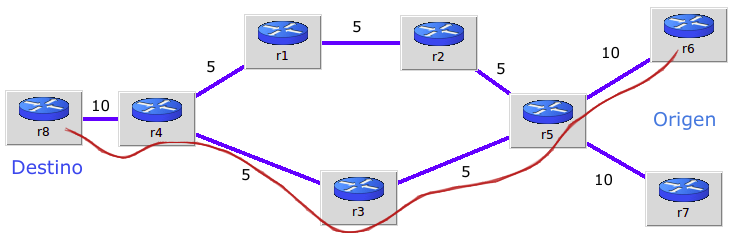
\includegraphics[width=0.93\textwidth]{Imagenes/pez.png}
	\caption{Problema del pez.}
\end{figure}

\vspace*{-2em}
El balanceador de carga con routing multicamino es uno de los casos de uso más comunes e implementados de SDN. 
\vspace{0.6em}

En nuestro caso, se desarrolla en un script en \textit{Python} que hemos llamado \texttt{multicamino.py}. %poner -> multicamino.py ??? o son demasiadas flechas en toda la presentación?
\vspace*{-2em}
\note{\large \vfill
	\begin{center}
		\begin{enumerate}
			\item Uno de los casos más implementados en SDN.
			\vspace{2em}	
            \item  	2 partes : BALANCEADOR - MULTICAMINO
			\vspace{2em}	
			\item SE NECESITAN LOS CAMINOS PARA APLICAR DESPUÉS EL BALANCEO ASÍ QUE EN EL ROUTING MULTICAMINO --> SIGUIENTE DIAPO.
			\vspace{2em}
			\vfill 
		\end{enumerate}
\end{center}}
\end{frame}



%%%%%%%%%%% Routing Multicamino
\begin{frame}{Routing multicamino}
\vspace*{-2em}
Técnica que explota los recursos de la red mediante la propagación del tráfico desde un nodo de origen a un nodo de destino por medio de múltiples rutas a lo largo de la red.
\begin{alertblock}{}
\begin{itemize}
\item Balanceo de carga
\item Agregación de ancho de banda.
\item Minimización de retardo de extremo a extremo.
\item Aumento de la tolerancia a fallos (mejorar fiabilidad).
\end{itemize}
\end{alertblock}
\note{\large \vfill
	\begin{center}
		\begin{enumerate}
			\item SE BASA EN LA PROPAGACIÓN DEL TRÁFICO DE UN NODO A OTRO POR MEDIO DE MULTIPLES RUTAS.
			\vspace{2em}	
			\item  E.G. balanceo, agregación de BW, Minimizar retardo, Aumentar tolerancia a fallos.
			\vspace{2em}
            \vfill
            
		\end{enumerate}
\end{center}}
\end{frame}


%%%%%%%%%%%%%%%%%%%%%%%%%%%% PathFinding Algorithms
\begin{frame}{PathFinding Algorithms}
\vspace*{-2em}
%Los algoritmos de \alert{\textbf{Pathing}} son los encargados de obtener la ruta más corta entre dos puntos. 
%\vspace*{-1em}
\begin{alertblock}{\small}
Los algoritmos de \alert{\textbf{Pathing}} son los encargados de obtener la ruta más corta entre dos puntos.
\begin{itemize}
\item DFS y BFS son dos algoritmos conocidos, que en la búsqueda agotan todas las posibilidades.
%\begin{itemize}
\item Iteran sobre todos los caminos posibles hasta alcanzar el nodo de destino
\item Se ejecutan en tiempo lineal, según la notación Big-$\mathcal{O}$ sería: $\mathcal{O}(N+E)$
%\end{itemize}
\end{itemize}
\end{alertblock}
\note{\large \vfill
	\begin{center}
		\begin{enumerate}
        	\item Se basan en encontrar la ruta más corta entre dos puntos
			\vspace{2em}
            \item  DFS BFS agotan todas las posibilidades.
			\item BFS-Búsqueda en Anchura, DFS-Búsqueda profundidad.
            \vspace{2em}	
			\item VENTAJA se EJECUTAN en TIEMPO LINEAL
			\vspace{2em}
       
			\vfill
		\end{enumerate}
\end{center}}
\end{frame}

%%%%%%%%%%%%%%%%%%%%%%%%%%%% Depth-first Search Algorithm (DFS)
\begin{frame}{Depth-first Search Algorithm (DFS)}
\vspace*{-2em}
\begin{alertblock}{\LARGE DFS}
\begin{itemize}
\item Búsqueda en profundidad del grafo.
\item Explora todos los nodos en un grafo hasta encontrar el nodo más profundo y después retrocede  con el propósito de encontrar otros posibles nodos.
\item Hace uso de una pila (\textit{stack}).
\end{itemize}
\end{alertblock}
\note{\large \vfill
	\begin{center}
		\begin{enumerate}
			\item ELEGIDO PARA ESTE TRABAJO, por el USO DE PILA
			\vspace{2em}	
			\item BUSQUEDA EN PROFUNDIDAD -> como se observa en la siguiente DIAPO.
			\vspace{2em}
			\vfill
		\end{enumerate}
\end{center}}
\end{frame}

%%%%%%%%%%%%%%%%%%%%%%%%%%%%  Iteraciones DFS
\begin{frame}{Iteraciones DFS}
\vspace*{-2.2em}
%% FIGURA DFS ----- REALIZADA EN https://www.mathcha.io/editor  
\begin{figure}[h!]
	\centering
	% \hspace*{-0.46in}% PARA AJUSTAR IZQ-DCH LA FIGURA.
	\resizebox{\textwidth}{!}{  % ESCALAR LA FIGURA, CON ESTE COMANDO SE QUE NO SE ME VA A SALIR FUERA DE TEXTWIDTH
		\tikzset{every picture/.style={line width=0.75pt}} %set default line width to 0.75pt        
		\begin{tikzpicture}[x=0.75pt,y=0.75pt,yscale=-1,xscale=1]
		%uncomment if require: \path (0,693.1666717529297); %set diagram left start at 0, and has height of 693.1666717529297
		
		\draw    (50, 39.36) rectangle (50, 39.36)   ;
		\draw    (384, 41.87) rectangle (384, 41.87)   ;
		\draw    (239, 11.12) rectangle (239, 11.12)   ;
		\draw    (54, 156.67) rectangle (54, 156.67)   ;
		\draw    (541, -39.33) rectangle (541, -39.33)   ;
		\draw    (384, 156.67) rectangle (384, 156.67)   ;
		\draw    (227, 127.19) rectangle (227, 127.19)   ;
		\draw    (54, 275.24) rectangle (54, 275.24)   ;
		\draw    (384, 275.24) rectangle (384, 275.24)   ;
		\draw    (227, 245.76) rectangle (227, 245.76)   ;
		
		\draw  [fill={rgb, 255:red, 244; green, 12; blue, 141 }  ,fill opacity=0.65 ]  (42, 45.22) circle [x radius= 10.97, y radius= 10.97]   ;
		\draw (42,45.21) node  [align=left] {\textbf{A}};
		\draw    (86, 12.58) circle [x radius= 10.63, y radius= 10.63]   ;
		\draw (86,12.59) node  [align=left] {B};
		\draw    (217, 16.35) circle [x radius= 10.63, y radius= 10.63]   ;
		\draw (217,16.35) node  [align=left] {E};
		\draw    (157, 54) circle [x radius= 10.97, y radius= 10.97]   ;
		\draw (157,53.99) node  [align=left] {D};
		\draw    (86, 81.6) circle [x radius= 10.97, y radius= 10.97]   ;
		\draw (86,81.6) node  [align=left] {C};
		\draw    (248, 45.22) circle [x radius= 10.97, y radius= 10.97]   ;
		\draw (248,45.21) node  [align=left] {G};
		\draw    (187, 97.92) circle [x radius= 10.31, y radius= 10.31]   ;
		\draw (187,97.91) node  [align=left] {F};
		\draw  [fill={rgb, 255:red, 244; green, 12; blue, 141 }  ,fill opacity=0.65 ]  (374, 45.22) circle [x radius= 10.63, y radius= 10.63]   ;
		\draw (374,45.21) node  [align=left] {A};
		\draw  [fill={rgb, 255:red, 45; green, 220; blue, 243 }  ,fill opacity=0.39 ]  (424, 13.85) circle [x radius= 10.97, y radius= 10.97]   ;
		\draw (424,13.84) node  [align=left] {\textbf{B}};
		\draw    (551, 18.87) circle [x radius= 10.63, y radius= 10.63]   ;
		\draw (551,18.86) node  [align=left] {E};
		\draw    (491, 56.5) circle [x radius= 10.97, y radius= 10.97]   ;
		\draw (491,56.5) node  [align=left] {D};
		\draw    (424, 82.85) circle [x radius= 10.97, y radius= 10.97]   ;
		\draw (424,82.85) node  [align=left] {C};
		\draw    (582, 47.72) circle [x radius= 10.97, y radius= 10.97]   ;
		\draw (582,47.72) node  [align=left] {G};
		\draw    (521, 100.42) circle [x radius= 10.31, y radius= 10.31]   ;
		\draw (521,100.42) node  [align=left] {F};
		\draw (20,68.9) node  [align=left] {\textbf{Origen}};
		\draw (273,67.76) node  [align=left] {\textbf{Destino}};
		\draw  [fill={rgb, 255:red, 244; green, 12; blue, 141 }  ,fill opacity=0.65 ]  (40, 158.13) circle [x radius= 10.63, y radius= 10.63]   ;
		\draw (40,158.14) node  [align=left] {A};
		\draw  [fill={rgb, 255:red, 25; green, 175; blue, 195 }  ,fill opacity=1 ]  (91, 129.9) circle [x radius= 10.63, y radius= 10.63]   ;
		\draw (91,129.91) node  [align=left] {B};
		\draw    (221, 133.67) circle [x radius= 10.63, y radius= 10.63]   ;
		\draw (221,133.67) node  [align=left] {E};
		\draw  [fill={rgb, 255:red, 45; green, 220; blue, 243 }  ,fill opacity=0.39 ]  (161, 171.32) circle [x radius= 10.97, y radius= 10.97]   ;
		\draw (161,171.31) node  [align=left] {\textbf{D}};
		\draw    (94, 197.67) circle [x radius= 10.97, y radius= 10.97]   ;
		\draw (94,197.66) node  [align=left] {C};
		\draw    (252, 162.53) circle [x radius= 10.97, y radius= 10.97]   ;
		\draw (252,162.53) node  [align=left] {G};
		\draw    (191, 217.73) circle [x radius= 10.31, y radius= 10.31]   ;
		\draw (191,217.74) node  [align=left] {F};
		\draw  [fill={rgb, 255:red, 244; green, 12; blue, 141 }  ,fill opacity=0.65 ]  (374, 160.02) circle [x radius= 10.63, y radius= 10.63]   ;
		\draw (374,160.02) node  [align=left] {A};
		\draw  [fill={rgb, 255:red, 25; green, 175; blue, 195 }  ,fill opacity=1 ]  (421, 129.9) circle [x radius= 10.63, y radius= 10.63]   ;
		\draw (421,129.91) node  [align=left] {B};
		\draw    (551, 133.67) circle [x radius= 10.63, y radius= 10.63]   ;
		\draw (551,133.67) node  [align=left] {E};
		\draw  [fill={rgb, 255:red, 25; green, 175; blue, 195 }  ,fill opacity=1 ]  (491, 171.32) circle [x radius= 10.97, y radius= 10.97]   ;
		\draw (491,171.31) node  [align=left] {D};
		\draw  [fill={rgb, 255:red, 45; green, 220; blue, 243 }  ,fill opacity=0.39 ]  (424, 197.67) circle [x radius= 10.97, y radius= 10.97]   ;
		\draw (424,197.66) node  [align=left] {\textbf{C}};
		\draw    (582, 162.53) circle [x radius= 10.97, y radius= 10.97]   ;
		\draw (582,162.53) node  [align=left] {G};
		\draw    (521, 217.73) circle [x radius= 10.31, y radius= 10.31]   ;
		\draw (521,217.74) node  [align=left] {F};
		\draw  [fill={rgb, 255:red, 244; green, 12; blue, 141 }  ,fill opacity=0.65 ]  (40, 276.7) circle [x radius= 10.63, y radius= 10.63]   ;
		\draw (40,276.71) node  [align=left] {A};
		\draw  [fill={rgb, 255:red, 25; green, 175; blue, 195 }  ,fill opacity=1 ]  (91, 248.48) circle [x radius= 10.63, y radius= 10.63]   ;
		\draw (91,248.48) node  [align=left] {B};
		\draw    (221, 252.23) circle [x radius= 10.63, y radius= 10.63]   ;
		\draw (221,252.24) node  [align=left] {E};
		\draw  [fill={rgb, 255:red, 25; green, 175; blue, 195 }  ,fill opacity=1 ]  (161, 289.88) circle [x radius= 10.97, y radius= 10.97]   ;
		\draw (161,289.88) node  [align=left] {D};
		\draw  [fill={rgb, 255:red, 25; green, 175; blue, 195 }  ,fill opacity=1 ]  (94, 316.23) circle [x radius= 10.97, y radius= 10.97]   ;
		\draw (94,316.23) node  [align=left] {C};
		\draw    (252, 281.1) circle [x radius= 10.97, y radius= 10.97]   ;
		\draw (252,281.1) node  [align=left] {G};
		\draw  [fill={rgb, 255:red, 45; green, 220; blue, 243 }  ,fill opacity=0.39 ]  (191, 336.3) circle [x radius= 10.31, y radius= 10.31]   ;
		\draw (191,336.31) node  [align=left] {\textbf{F}};
		\draw  [fill={rgb, 255:red, 244; green, 12; blue, 141 }  ,fill opacity=0.65 ]  (374, 278.58) circle [x radius= 10.63, y radius= 10.63]   ;
		\draw (374,278.59) node  [align=left] {A};
		\draw  [fill={rgb, 255:red, 25; green, 175; blue, 195 }  ,fill opacity=1 ]  (421, 248.48) circle [x radius= 10.63, y radius= 10.63]   ;
		\draw (421,248.48) node  [align=left] {B};
		\draw    (551, 252.23) circle [x radius= 10.63, y radius= 10.63]   ;
		\draw (551,252.24) node  [align=left] {E};
		\draw  [fill={rgb, 255:red, 25; green, 175; blue, 195 }  ,fill opacity=1 ]  (491, 289.88) circle [x radius= 10.97, y radius= 10.97]   ;
		\draw (491,289.88) node  [align=left] {D};
		\draw  [fill={rgb, 255:red, 25; green, 175; blue, 195 }  ,fill opacity=1 ]  (424, 316.23) circle [x radius= 10.97, y radius= 10.97]   ;
		\draw (424,316.23) node  [align=left] {C};
		\draw  [fill={rgb, 255:red, 126; green, 211; blue, 33 }  ,fill opacity=0.7 ]  (582, 281.1) circle [x radius= 10.97, y radius= 10.97]   ;
		\draw (582,281.1) node  [align=left] {\textbf{G}};
		\draw  [fill={rgb, 255:red, 25; green, 175; blue, 195 }  ,fill opacity=1 ]  (521, 336.3) circle [x radius= 10.31, y radius= 10.31]   ;
		\draw (521,336.31) node  [align=left] {F};
		\draw (610,303.27) node  [align=left] {\textbf{Destino}};
		\draw (350,303.27) node  [align=left] {\textbf{Origen}};
		\draw  [fill={rgb, 255:red, 244; green, 12; blue, 141 }  ,fill opacity=0.65 ]   (126.33, 370.97) rectangle (153.67, 390.7)   ;
		\draw (140,380.83) node  [align=left] { \ A };
		\draw  [fill={rgb, 255:red, 126; green, 211; blue, 33 }  ,fill opacity=0.7 ]   (465.67, 370.97) rectangle (494.33, 390.7)   ;
		\draw (480,380.83) node  [align=left] { \ G };
		\draw  [fill={rgb, 255:red, 45; green, 220; blue, 243 }  ,fill opacity=0.39 ]   (395, 370.97) rectangle (425, 390.7)   ;
		\draw (410,380.83) node  [align=left] { \ \ F };
		\draw  [fill={rgb, 255:red, 45; green, 220; blue, 243 }  ,fill opacity=0.39 ]   (191.33, 370.97) rectangle (218.67, 390.7)   ;
		\draw (205,380.83) node  [align=left] { \ B };
		\draw  [fill={rgb, 255:red, 45; green, 220; blue, 243 }  ,fill opacity=0.39 ]   (257, 370.97) rectangle (285, 390.7)   ;
		\draw (271,380.83) node  [align=left] { \ D };
		\draw  [fill={rgb, 255:red, 45; green, 220; blue, 243 }  ,fill opacity=0.39 ]   (327, 370.97) rectangle (355, 390.7)   ;
		\draw (341,380.83) node  [align=left] { \ C };
		\draw    (50.45,52.2) -- (77.55,74.61) ;
		
		
		\draw    (50.81,38.68) -- (77.46,18.92) ;
		
		
		\draw    (95.18,17.94) -- (147.53,48.47) ;
		
		
		\draw    (96.63,12.89) -- (206.37,16.05) ;
		
		
		\draw    (146.78,57.97) -- (96.22,77.63) ;
		
		
		\draw    (166.29,48.17) -- (208,22) ;
		
		
		\draw    (224.78,23.59) -- (239.98,37.74) ;
		
		
		\draw    (239.7,52.38) -- (194.8,91.17) ;
		
		
		\draw    (176.83,96.27) -- (96.83,83.35) ;
		
		
		\draw    (382.5,51.61) -- (415.24,76.26) ;
		
		
		\draw    (383,39.56) -- (414.71,19.67) ;
		
		
		\draw    (433.25,19.74) -- (481.75,50.61) ;
		
		
		\draw    (434.96,14.28) -- (540.38,18.44) ;
		
		
		\draw    (480.8,60.52) -- (434.21,78.84) ;
		
		
		\draw    (500.29,50.68) -- (541.99,24.51) ;
		
		
		\draw    (558.78,26.11) -- (573.97,40.25) ;
		
		
		\draw    (573.7,54.89) -- (528.8,93.68) ;
		
		
		\draw    (510.86,98.58) -- (434.79,84.81) ;
		
		
		\draw    (48.58,164.41) -- (85.15,191.19) ;
		
		
		\draw    (49.3,152.99) -- (81.7,135.05) ;
		
		
		\draw    (100.15,135.32) -- (151.56,165.73) ;
		
		
		\draw    (101.63,130.21) -- (210.37,133.36) ;
		
		
		\draw    (150.79,175.32) -- (104.2,193.65) ;
		
		
		\draw    (170.29,165.48) -- (212,139.32) ;
		
		
		\draw    (228.78,140.91) -- (243.98,155.06) ;
		
		
		\draw    (243.87,169.89) -- (198.64,210.82) ;
		
		
		\draw    (180.91,215.65) -- (104.74,199.88) ;
		
		
		\draw    (382.49,166.41) -- (415.24,191.07) ;
		
		
		\draw    (382.95,154.28) -- (412.05,135.64) ;
		
		
		\draw    (430.15,135.32) -- (481.56,165.73) ;
		
		
		\draw    (431.63,130.21) -- (540.37,133.36) ;
		
		
		\draw    (480.79,175.32) -- (434.2,193.65) ;
		
		
		\draw    (500.29,165.48) -- (542,139.32) ;
		
		
		\draw    (558.78,140.91) -- (573.98,155.06) ;
		
		
		\draw    (573.87,169.89) -- (528.64,210.82) ;
		
		
		\draw    (510.91,215.65) -- (434.74,199.88) ;
		
		
		\draw    (48.57,282.98) -- (85.15,309.76) ;
		
		
		\draw    (49.3,271.56) -- (81.7,253.63) ;
		
		
		\draw    (100.15,253.89) -- (151.56,284.3) ;
		
		
		\draw    (101.63,248.78) -- (210.37,251.93) ;
		
		
		\draw    (150.79,293.9) -- (104.2,312.22) ;
		
		
		\draw    (170.29,284.05) -- (212,257.89) ;
		
		
		\draw    (228.78,259.48) -- (243.97,273.63) ;
		
		
		\draw    (243.87,288.46) -- (198.65,329.39) ;
		
		
		\draw    (180.9,334.22) -- (104.74,318.45) ;
		
		
		\draw    (382.49,284.98) -- (415.24,309.64) ;
		
		
		\draw    (382.95,272.85) -- (412.05,254.21) ;
		
		
		\draw    (430.15,253.89) -- (481.56,284.3) ;
		
		
		\draw    (431.63,248.78) -- (540.37,251.93) ;
		
		
		\draw    (480.79,293.9) -- (434.2,312.22) ;
		
		
		\draw    (500.29,284.05) -- (542,257.89) ;
		
		
		\draw    (558.78,259.48) -- (573.97,273.63) ;
		
		
		\draw    (573.87,288.46) -- (528.65,329.39) ;
		
		
		\draw    (510.9,334.22) -- (434.74,318.45) ;
		
		
		\draw    (425,380.83) -- (465.67,380.83) ;
		\draw [shift={(465.67,380.83)}, rotate = 180] [color={rgb, 255:red, 0; green, 0; blue, 0 }  ]   (0,0) .. controls (3.31,-0.3) and (6.95,-1.4) .. (10.93,-3.29)(0,0) .. controls (3.31,0.3) and (6.95,1.4) .. (10.93,3.29)   ;
		
		\draw    (153.67,380.83) -- (191.33,380.83) ;
		\draw [shift={(191.33,380.83)}, rotate = 180] [color={rgb, 255:red, 0; green, 0; blue, 0 }  ]   (0,0) .. controls (3.31,-0.3) and (6.95,-1.4) .. (10.93,-3.29)(0,0) .. controls (3.31,0.3) and (6.95,1.4) .. (10.93,3.29)   ;
		
		\draw    (218.67,380.83) -- (257,380.83) ;
		\draw [shift={(257,380.83)}, rotate = 180] [color={rgb, 255:red, 0; green, 0; blue, 0 }  ]   (0,0) .. controls (3.31,-0.3) and (6.95,-1.4) .. (10.93,-3.29)(0,0) .. controls (3.31,0.3) and (6.95,1.4) .. (10.93,3.29)   ;
		
		\draw    (285,380.83) -- (327,380.83) ;
		\draw [shift={(327,380.83)}, rotate = 180] [color={rgb, 255:red, 0; green, 0; blue, 0 }  ]   (0,0) .. controls (3.31,-0.3) and (6.95,-1.4) .. (10.93,-3.29)(0,0) .. controls (3.31,0.3) and (6.95,1.4) .. (10.93,3.29)   ;
		
		\draw    (355,380.83) -- (395,380.83) ;
		\draw [shift={(395,380.83)}, rotate = 180] [color={rgb, 255:red, 0; green, 0; blue, 0 }  ]   (0,0) .. controls (3.31,-0.3) and (6.95,-1.4) .. (10.93,-3.29)(0,0) .. controls (3.31,0.3) and (6.95,1.4) .. (10.93,3.29)   ;
		\end{tikzpicture}
	}	
	\caption{Iteraciones del algoritmo DFS.}
	\label{fig: DFS}
\end{figure}
\note{\large \vfill
	\begin{center}
		\begin{enumerate}
			\item ITERACIONES DFS hasta encontrar el destino.
			\vspace{2em}	
			\item En orden descendiente, se visita el vecino del origen, despues el vecino del vecino..
			\vspace{2em}	
			\item NO ACABA AQUÍ,  se volvería atrás al ultimo nodo que queda en la pila (E).
			\vspace{2em}
            
			\vfill
		\end{enumerate}
\end{center}}
\end{frame}


%%%%%%%%%%%%%%%%%%%%%%%%%%%% Cálculo del coste por camino
\begin{frame}{Cálculo del coste por camino}
\vspace*{-2em}
\begin{alertblock}{\large DFS devuelve una lista con las rutas, pero sin pesos.}
\vspace*{1em}
Tenemos que medir el coste de los caminos o rutas:
\begin{enumerate}
\item Calcular todos los costes de enlaces que haya en la ruta.\\ \vspace*{0.5em}  {\large $Cost(l) = \frac{BW_{Reference}}{BW(l)}\quad\mathrm{;}\quad$} 
\\ \vspace*{0.5em} {\large $BW(l) = min\hspace{0.4em}(\hspace{0.2em}BW_{Switch1}, BW_{Switch2}\hspace{0.2em})$}
\vspace{1em}
\item Calcular el coste total de la ruta (sumar los costes de enlaces).
\end{enumerate}
\end{alertblock}
\note{\large \vfill
	\begin{center}
		\begin{enumerate}
			\item DFS DEVUELVE LAS RUTAS, PERO SIN PESOS. 
			\vspace{2em}
			\item Calculamos el coste como en OSPF (protocolo de red) 
			\vspace{2em}	
			\item  BW enlace = BW de la interfaz de un switch.
			\vspace{2em}
			\item  COSTE DE ENLACE = 1 -> COSTE DE LA RUTA ES EL Nº DE ENLACES (FÁCIL PARA ENTENDERLO).
			\vspace{2em}
			\vfill
		\end{enumerate}
\end{center}}
\end{frame}



%%%%%%%%%%%%%%%%%%%%%%%%%%%%  Bucket weight en OpenFlow
\begin{frame}{Bucket weight en OpenFlow}
\vspace*{-0.1em}
\begin{alertblock}{\large \emph{Group}\rightarrow \emph{Group table}\rightarrow \emph{buckets (bucket weight)}\rightarrow \emph{acciones}}
\vspace*{1em}
\begin{wrapfigure}{l}{0.45\textwidth}
	\centering
	\vspace{-1.5em}
	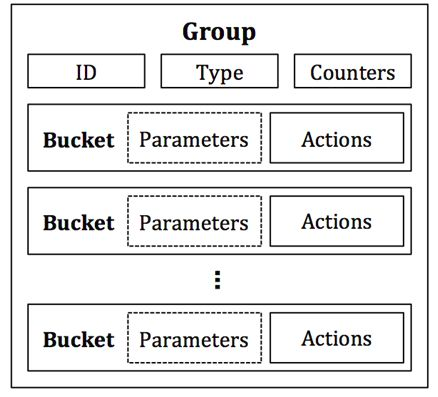
\includegraphics[width=0.45\textwidth]{figuras/gruposs.png}
	\caption{Grupo OpenFlow.}
	\label{img: grupo_openflow}
	\vspace*{-0.8em}
\end{wrapfigure}
Los \emph{Grupos} en OpenFlow representan una serie de puertos como una entidad única para el envío de paquetes. Existen varios tipos de grupos, interesándonos los \emph{Select} para el multicamino. 
\vspace*{1em}

\large$bw(p) = \left( 1 - \frac{Cost(p)}{\sum_{i=0}^{i<n} Cost(i)}\right)\times{10}$
\end{alertblock}
\note{\large \vfill
	\begin{center}
		\begin{enumerate}
		    \item Openflow no entiende costes, sino BUCKET WEIGHTS, CONTRARIOS AL COSTE.
			\vspace{2em}
            \item Tenemos por tanto que solucionar el problema que nos surge, ajustar el criterio
de los bucket weights con los costes de las ruta.	\vspace{2em}
            \item Una vez ajustado el cambio, toca la implementación-->SIGUIENTE DIAPO.
			\vspace{2em}
			\vfill
		\end{enumerate}
\end{center}}
\end{frame}






%%%%%%%%%%%%%%%%%%%%%%%%%%%%%%%%%%%%%%%%%%%%%%%
%% SECCIÓN NUEVA: Conclusiones y líneas futuras
%%%%%%%%%%%%%%%%%%%%%%%%%%%%%%%%%%%%%%%%%%%%%%%

\section{Implementación}

%%%%%%%%%%%%%%%%%%%%%%%%%%%% Requirements
\begin{frame}{Requisitos}
\vspace*{-2em}
\begin{exampleblock}{\LARGE Requisitos}
\begin{center}
\begin{enumerate}
\large
\item Máquina corriendo \texttt{Ubuntu 16.04.3} o superior.
\vspace*{0.5em}
\item \texttt{Mininet v2.2.2} o superior.
\vspace*{0.5em}
\item \texttt{Ryu v4.0} o superior. 
\vspace*{0.5em}
\item \texttt{iPerf} \end{enumerate}
\end{center}
\end{exampleblock}
\note{\large \vfill
	\begin{center}
		\begin{enumerate}
			\item  Requisitos necesarios para realizar el experimento.
			\vspace{2em}	
			\item  Que tenga miniedit.
			\vspace{2em}
			\item  Actualizaciones en la API.
            \vspace{2em}
            \vfill 
            
		\end{enumerate}
\end{center}}
\end{frame}




%%%%%%%%%%%%%%%%%%%%%%%%%%%%  ENTORNO DE DESARROLLO
\begin{frame}{Entorno de desarrollo}
\vspace*{2em}
\begin{figure}[h!]
	\centering
	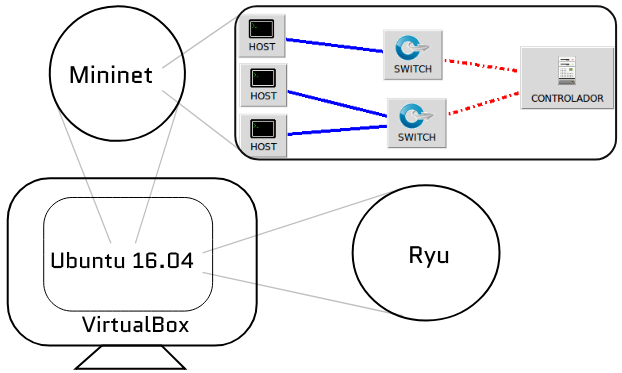
\includegraphics[width=0.93\textwidth]{figuras/entorno_de_desarrollo.png}
	\caption{Entorno de desarrollo.}
	\label{img: entorno_de_desarrollo}
\end{figure}

\note{\large \vfill
	\begin{center}
		\begin{enumerate}
			\item De dentro a fuera (MININET->RYU->UBUNTU->VBOX..)
			\vspace{2em}
			\item igual para los dos casos de uso
			\vspace{2em}	
            \vfill
		\end{enumerate}
\end{center}}
\end{frame}




%%%%%%%%%%%%%%%%%%%%%%%%%%%%  Balanceador de carga multicamino I
\begin{frame}{Balanceador de carga multicamino I}
\vspace*{-1em}
\begin{exampleblock}{\centering \large Definición del escenario de aplicación}
\end{exampleblock}
%\begin{figure}[h!]
%	\centering
%	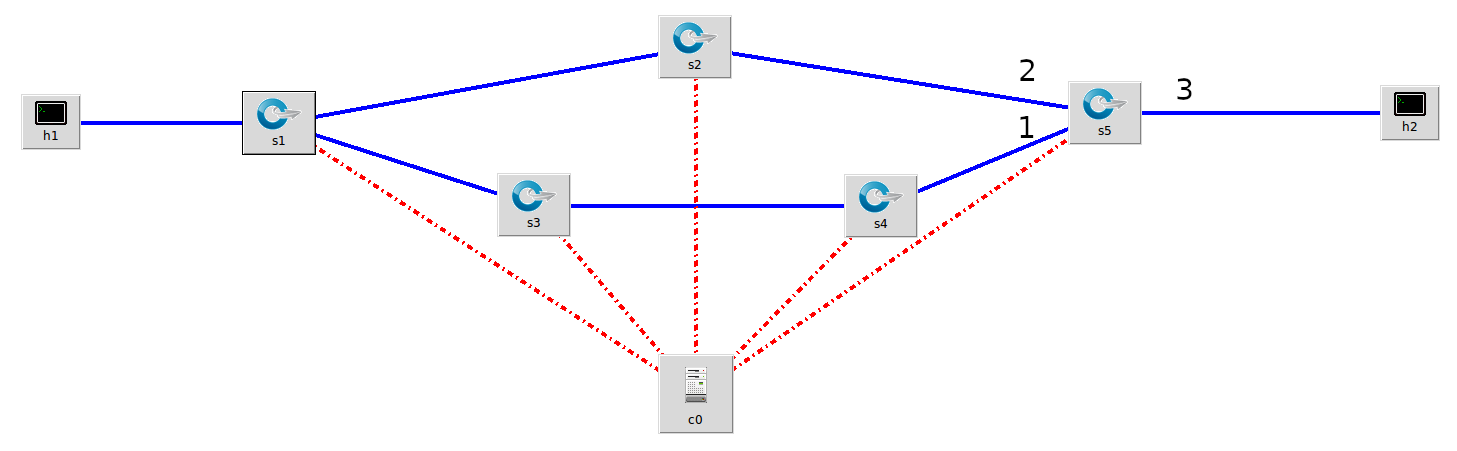
\includegraphics[width=1\textwidth]{Imagenes/topologia_multicamino_puertos.png}
%	\caption{Topología elegida para el routing multicamino con balanceo de carga.}
%\end{figure}
\begin{figure}[!h]
    \centering

\noindent\makebox[\textwidth][l]{%
  \hspace{-\dimexpr\oddsidemargin+1in}%
  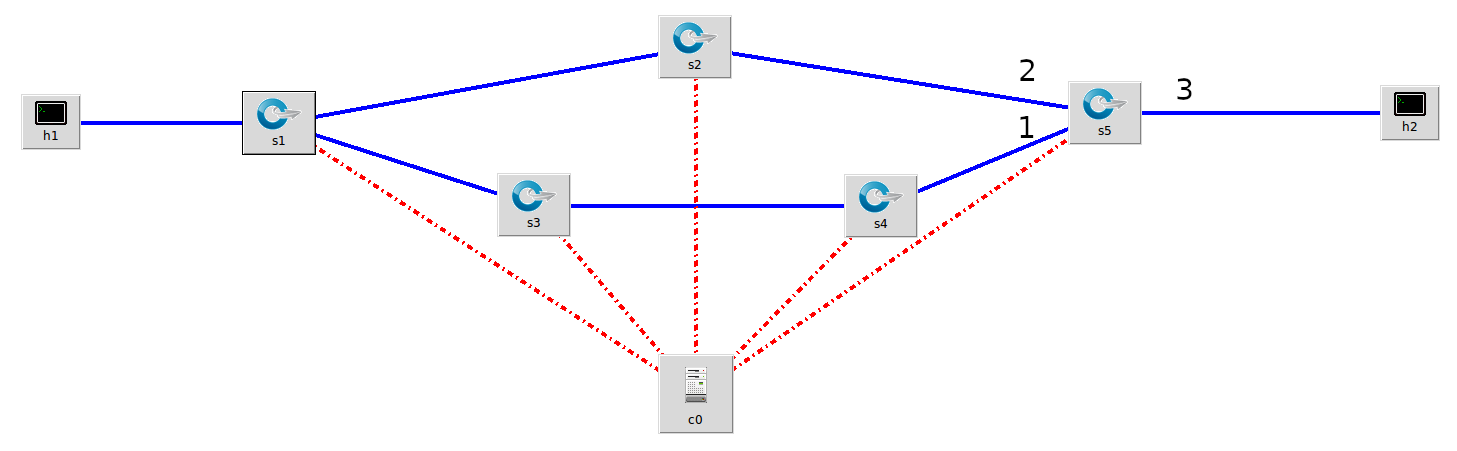
\includegraphics[width=\paperwidth]{Imagenes/topologia_multicamino_puertos.png}%
}
\end{figure}




\note{\large \vfill
	\begin{center}
		\begin{enumerate}
			\item  \textcolor{red}{SOLUCIONAR PROBLEMA CON EL FONDO BLANCO DE LA CAPTURA DE MINIEDIT.}
			\vspace{2em}	
			\item  Primer caso de uso.
			\vspace{2em}
			\item  Diseñamos en Miniedit y configuramos el controlador. IP  loopback, puerto 6633, remote controller y OpenFlow 1.3
			\vspace{2em}
			\vfill
		\end{enumerate}
\end{center}}
\end{frame}


%%%%%%%%%%%%%%%%%%%%%%%%%%%%  Balanceador de carga multicamino II
{\nologo
\begin{frame}{Balanceador de carga multicamino II} 
	\vspace*{0.5em}
    \begin{exampleblock}{\centering Inicio del controlador y descubrimiento de rutas}
%	\begin{figure}[h!]			
%			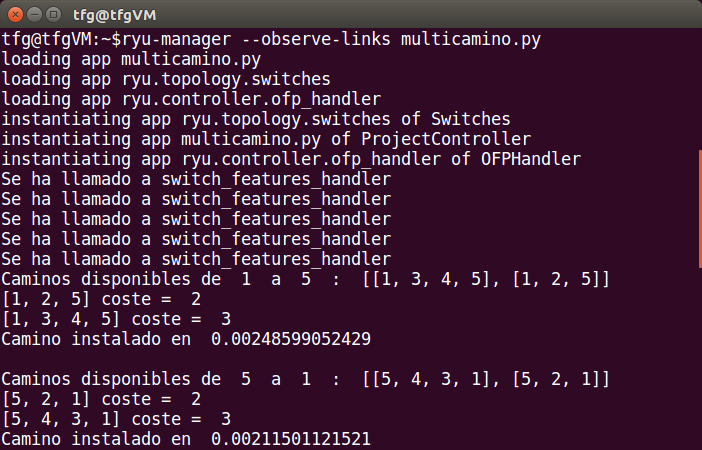
\includegraphics[width=0.9\textwidth]{Imagenes/miniedit_multicamino_descubrimiento_de_rutas.png}
%		\end{figure}

	\end{exampleblock}
	\begin{figure}[!h]
    	\centering
		\noindent\makebox[\textwidth][r]{%
  		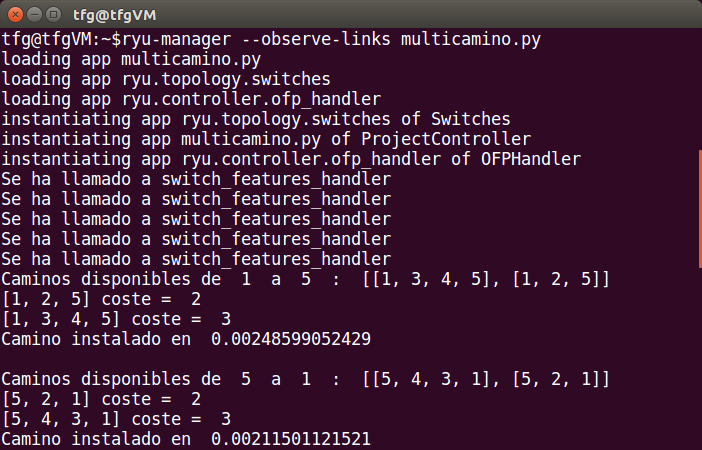
\includegraphics[width=0.85\paperwidth]{Imagenes/miniedit_multicamino_descubrimiento_de_rutas.png}%
}
	\end{figure}
		




\note{\large \vfill
	\begin{center}
		\begin{enumerate}
			\item  Una vez diseñada la topología, iniciamos el controlador para que descubra las rutas.
			\vspace{2em}	
			\item Las rutas se descubren hasta que no se realiza un ping H1-H2
			\vspace{2em}	
			\item ir a la diapo anterior y que las rutas concuerdan.
			\vspace{2em}
			\item  Salen los caminos de ida y vuelta porque suponíamos que eran bidireccionales
			\vspace{2em}
			\vfill
		\end{enumerate}
\end{center}}
\end{frame}
} %fin de \nologo


%%%%%%%%%%%%%%%%%%%%%%%%%%%%  Balanceador de carga multicamino III
\begin{frame}{Balanceador de carga multicamino III}
\vspace*{2em}
\begin{figure}[h!]
	\centering
	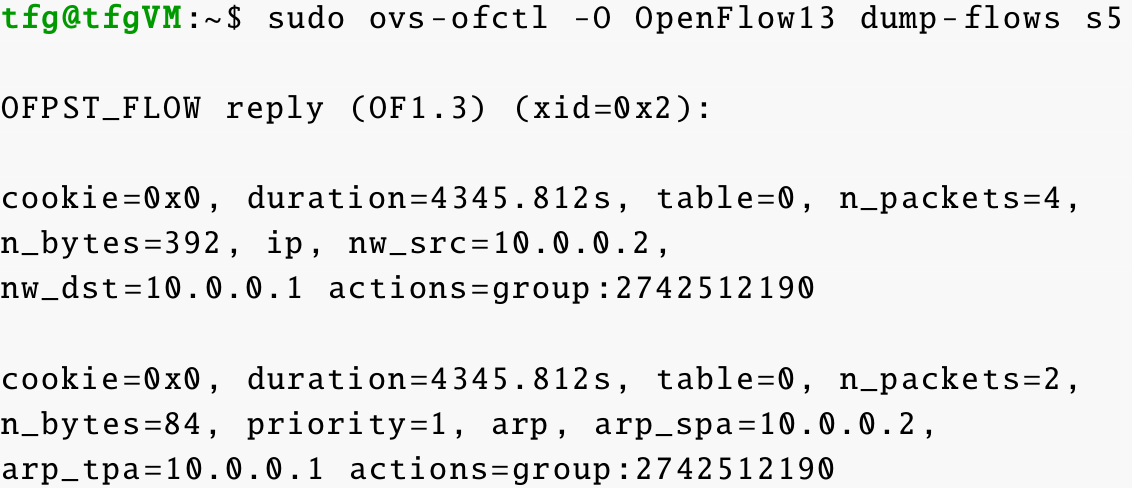
\includegraphics[width=1\textwidth]{Imagenes/flows.png}
\end{figure}


\note{\large \vfill
	\begin{center}
		\begin{enumerate}
        \item  veamos si las rutas HAN SIDO INSTALADAS EN S5. Este es el primer paso. haremos flows->grupos-> buckets->actions
			\vspace{2em}
	        \item Cada flow se encarga del matching de pkts IP y ARP (uno de cada)
            \vspace{2em}
            \item Se ridirigen los dos al mismo grupo:-> Siguiente DIAPO
			
            \vspace{2em}	
			\vfill
		\end{enumerate}
\end{center}}
\end{frame}



{\nologo %quito el logo porque queda cortado con la imagen.
\begin{frame}{Balanceador de carga multicamino IV}
\vspace*{-0.7em}
\begin{figure}[!h]
    \centering

\noindent\makebox[\textwidth][l]{%
  \hspace{-\dimexpr\oddsidemargin+1in}%
  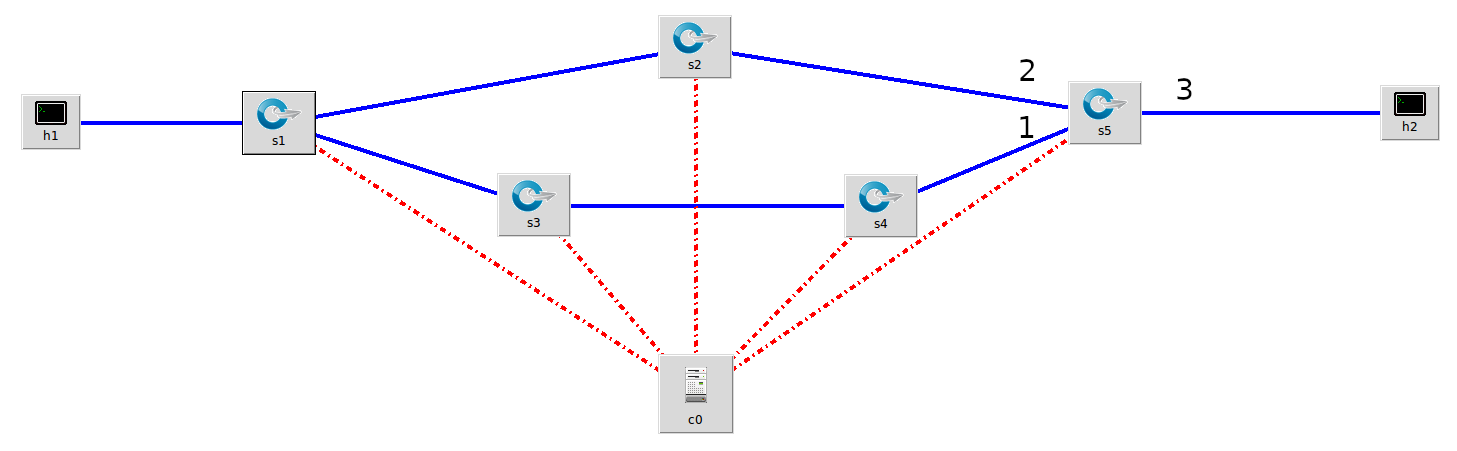
\includegraphics[width=\paperwidth]{Imagenes/topologia_multicamino_puertos.png}%
}
\end{figure}

\begin{figure}[h!]
	\centering
	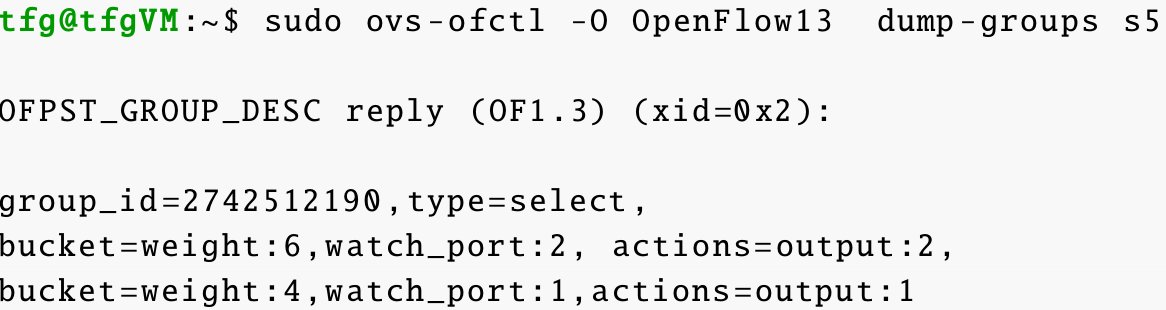
\includegraphics[width=1\textwidth]{Imagenes/groups.png}
\end{figure}
\note{\large \vfill
	\begin{center}
		\begin{enumerate}
			\item Este es el grupo, que tiene 2 buckets en la Group Table.
			\vspace{2em}	
			\item bucket weight se corresponde con el coste: 2/3=4/6
			\vspace{2em}
            	\item UNA VEZ COMPROBADO TODO --> CREAMOS TRÁFICO (SIGUIENTE DIAPO).
			\vspace{2em}
			\vfill
		\end{enumerate}
\end{center}}
\end{frame}
} %fin de \nologo

%%%%% PARA IR MOSTRANDO LAS RUTAS, SUS COSTES Y DEMÁS. 1 A 1.
%\begin{itemize}[<+- | alert@+>]
%\item 
%\item Now this
%\end{itemize}



%%%%%%%%%%%%%%%%%%%%%%%%%%%%  Balanceador de carga multicamino IV
{\nologo % quitamos el logo porque con la figura queda 
\begin{frame}{Balanceador de carga multicamino V}
\vspace*{-2em}
\begin{exampleblock}{\centering Creación de tráfico TCP con iPerf.}

\end{exampleblock}

\begin{figure}[h!]
	\centering	
	\par
\noindent\makebox[\textwidth][l]{%
  \hspace{-\dimexpr\oddsidemargin+1in}%
  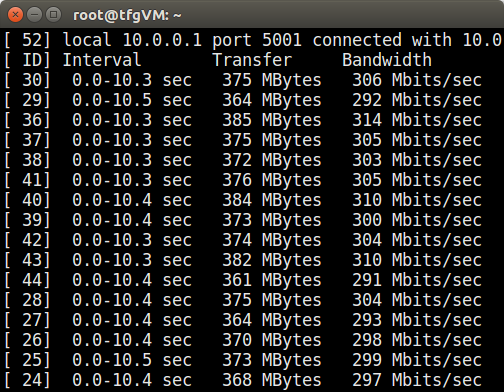
\includegraphics[width=0.5\paperwidth]{Imagenes/iperf2_server.png}%
  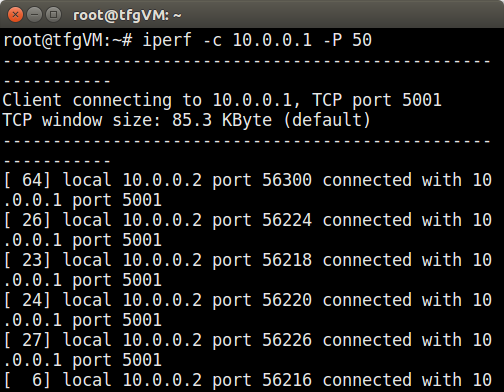
\includegraphics[width=0.5\paperwidth]{Imagenes/iperf2_client.png}%
}
	\par
\end{figure}
% \begin{figure}[h!]
% 	\centering	
% 	\par
% 	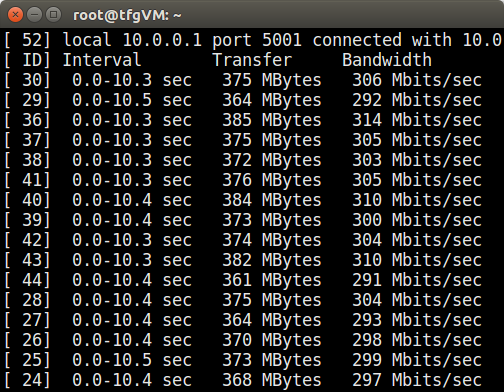
\includegraphics[width=0.49\textwidth]{Imagenes/iperf2_server.png}
% 	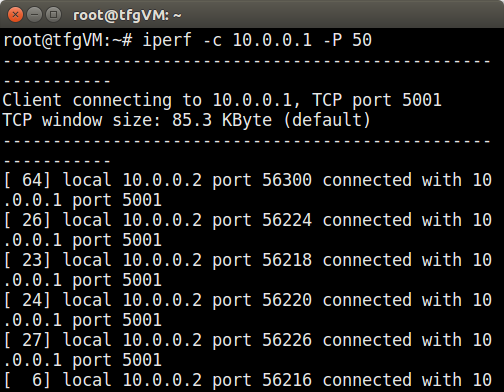
\includegraphics[width=0.49\textwidth]{Imagenes/iperf2_client.png}
% 	%\hfill
% 	\par
% 	\caption{Captura del envío de tráfico entre cliente y servidor iPerf.}
% 	\label{img: iperf1}
% \end{figure}

\note{\large \vfill
	\begin{center}
		\begin{enumerate}
			\item  Creamos tráfico TCP con iPerf. 50 clientes en paralelo.
			\vspace{2em}	 
			\item  si solo usamos un cliente, se usaría una sola ruta y no podriamos balancear. 
			\vspace{2em}
			\item  mirando la figura de la derecha (CLIENTE) se ve como se conectan los clientes cada uno con su puerto (port 56300, port 56224,...)
			\vspace{2em}
			\item  Una vez creado trafico --> COMPROBAMOS BALANCEO (SIGUIENTE DIAPO)
			\vspace{2em}
			\vfill
		\end{enumerate}
\end{center}}
\end{frame}
} %fin de \nologo





{\nologo %quito el logo porque queda cortado con la imagen.
\begin{frame}{Balanceador de carga multicamino VI}
\begin{exampleblock}{\centering \large Comprobación del balanceo de carga.}
\vspace*{-0.5em}
\begin{figure}[h!]
	\centering
	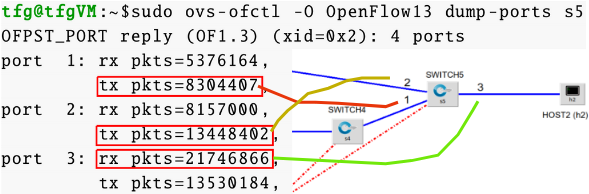
\includegraphics[width=1\textwidth]{Imagenes/untitled3.png}
\end{figure}
%%%%% PARA IR MOSTRANDO LAS RUTAS, SUS COSTES Y DEMÁS. 1 A 1.
\end{exampleblock}
\vspace*{-2em}
\begin{center}
	\begin{description}%[<+- | alert@+>] % para mostar uno a uno.
		\large
		\item[\textit{Ruta 1}]  $Traffic(1)=\frac{Tx2}{Rx3}\times{100}=62\% $
	
		\item[\textit{Ruta 2}] $Traffic(2)=\frac{Tx1}{Rx3}\times{100}=38\% $
	\end{description}
\end{center}

\note{\large \vfill
	\begin{center}
		\begin{enumerate}
			\item  se reciben por el puerto3 y se envian por los otros dos (p3=p1+p2)
			\vspace{2em}	
			\item El resultado se asemeja al teórico 4/10,6/10. sabiendo que una pequeña fracciñón del tráfico es creado por las comunicaciones entres switches. 
			\vspace{2em}
			\item  CONCLUSION: Se ha implementado correctamente el LB.
			\vspace{2em}
			\vfill
		\end{enumerate}
\end{center}}
\end{frame}
} %fin de \nologo









%%%%%%%%%%%%%% MONITORIZACIÓN DEL TRÁFICO CON CIERTA QoS I
%{\nologo %quito el logo porque queda cortado con la imagen.
\begin{frame}{Monitorización del tráfico con cierta QoS I}
%\begin{exampleblock}{\centering Comprobación del balanceo de carga.}

	Hoy en día la mayoría de las redes hacen uso de la calidad de servicio. 
    \begin{itemize}
    \item[\rightarrow] SDN debe ofrecer al menos
los mismos servicios y aplicaciones que las redes tradicionales.

    \end{itemize}
    
\begin{table}[h]
	\begin{threeparttable}
		\begin{tabular*}{\textwidth}{
				@{\extracolsep{\fill}\hspace{\tabcolsep}}
				l
				c
				c
				c
				c
				c
				c
				@{\hspace{\tabcolsep}}
			}
			\toprule
			& \multicolumn{2}{c}{Fase 1} & \multicolumn{2}{c}{Fase 2}  & \multicolumn{2}{c}{Fase 3} \\
			\cmidrule(lr){2-3} \cmidrule(lr){4-5} \cmidrule(lr){6-7}
			Tarifa				  & Datos         		& Tasa   		    & Datos    		& Tasa		   		& Datos   		   	& Tasa  			 \\
			\midrule
			Estándar              & \SI{2}{MB}   		& \SI{1}{Mbps}    	& \SI{1}{MB}  	& \SI{.2}{Mbps}    	&  --				& --      			 \\
			\addlinespace
			Premium               & $\infty$           	& \SI{2}{Mbps}      & $\infty$      & \SI{2}{Mbps}      & $\infty$          & \SI{2}{Mbps}       \\
			\addlinespace
			\bottomrule
		\end{tabular*}

	\end{threeparttable}
	\label{tab: fases_tarifas}
    \caption[Tarifas móviles y sus fases en función del consumo de datos.]
	{Tarifas móviles y sus fases en función del consumo de datos.}
	
\end{table}
\note{\large \vfill
	\begin{center}
		\begin{enumerate}
			\item Caso de uso incorpora QoS para ver que fácil se implementa en SDN.
			\vspace{2em}
            \item se pretende mostrar como se pueden transferir los datos de una red en función de la prioridad basada en el origen de los datos (usuarios).
       		\vspace{2em}	
            \item además reservar ancho de banda para una comunicación con el objetivo de unir dos puntos con un constante ancho de banda.		
            \vspace{2em}	
            \item Se implementa la tarifa ESTANDAR ya que es la más compleja.
            %\item[ESTANDAR]\textbf{1a fase}: 2 MB de datos a 1 Mbps. \textbf{2a fase}: 2 MB se reduce el 80\% para el siguiente 1 MB. \textbf{3a fase}: gastando los 3 MB, se queda sin poder transmitir ni recibir datos (i.e. la velocidad será 0 Kbps)
			%\item[PREMIUM] Datos ilimitados todo el mes, Vmin=2Mbps.
			\vspace{2em}
			\vfill
		\end{enumerate}
\end{center}}
\end{frame}
%} %fin de \nologo



%%%%%%%%%%%%%% MONITORIZACIÓN DEL TRÁFICO CON CIERTA QoS II
\begin{frame}{Monitorización del tráfico con cierta QoS II}
\vspace*{2em}
\begin{exampleblock}{\large Uso de Colas en OpenFlow}
\vspace*{1em}
Cada cola se corresponde con una fase de la tarifa, por lo que se crean tres colas, cada una con un id diferente.
\begin{itemize}
\item[\rightarrow] Se establece el cambio entre las fases mediante programación.
\end{itemize}
Prioridades de las colas:
\begin{description}
\item[Cola 0]{Prioridad 0}
\item[Cola 1]{Prioridad 1}
\item[Cola 2]{Prioridad 2}
\end{description}

\end{exampleblock}
\note{\large \vfill
	\begin{center}
		\begin{enumerate}
			\item  Para llevarlo a la práctica, se hace uso de las colas o queues en OpenFlow.
			\vspace{2em}	
			\item En el script se supone que ya existen y están configuradas dichas colas (las creamos antes de ejecutar el script).

			\vspace{2em}
			\item  Las prioridades hacen que por eso se empiece en la cola 0 y se vaya cambiando a la 1 y a la 2.
			\vspace{2em}	
            \item  \textcolor{red}{SE INICIA EL CONTROLADOR IGUAL QUE EN EL OTRO CASO PERO CON TARIFAS.PY}
			\vspace{2em}
			\vfill
		\end{enumerate}
\end{center}}
\end{frame}








%%%%%%%%%%%%%% MONITORIZACIÓN DEL TRÁFICO CON CIERTA QoS III
{\nologo %quito el logo porque queda cortado con la imagen.
\begin{frame}{Monitorización del tráfico con cierta QoS III}
%\begin{exampleblock}{\centering Comprobación del balanceo de carga.}
\vspace*{1.5em}
\begin{figure}[h!]
	%\centering
	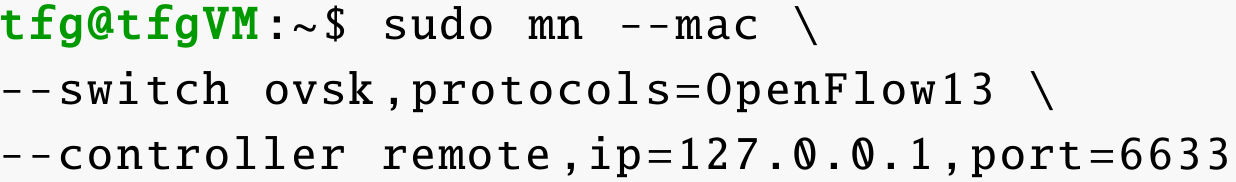
\includegraphics[width=0.8\textwidth,left]{Imagenes/arrancar_mininet.png}
\end{figure}
\begin{figure}[h!]
	\centering
	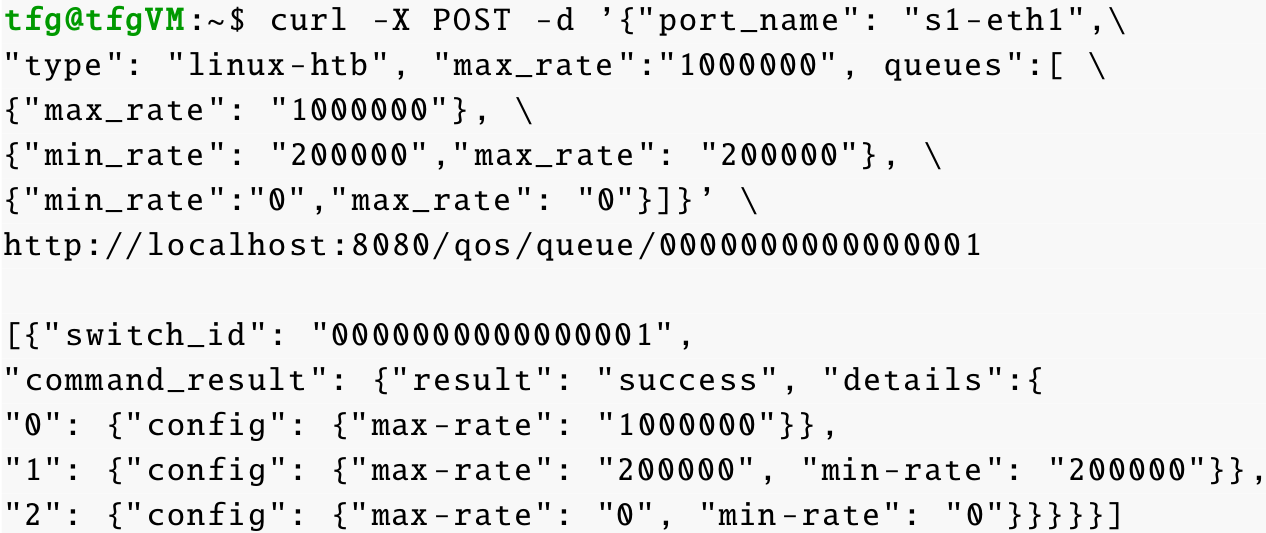
\includegraphics[width=1\textwidth]{Imagenes/colas.png}
\end{figure}
%%%%% PARA IR MOSTRANDO LAS RUTAS, SUS COSTES Y DEMÁS. 1 A 1.

%\end{exampleblock}
\note{\large \vfill
	\begin{center}
		\begin{enumerate}
			\item  Toca por tanto, arrancar Mininet y configurar las colas
			\vspace{2em}	
			\item 3 colas, 1Mbps, 200ks, 0. (tarifa standar)
			\vspace{2em}
			\item  Output del comando nos devuelve SUCCESS (exito).
			\vspace{2em}
			\vfill
		\end{enumerate}
\end{center}}
\end{frame}
} %fin de \nologo





%%%%%%%%%%%%%% MONITORIZACIÓN DEL TRÁFICO CON CIERTA QoS IV
\begin{frame}{Monitorización del tráfico con cierta QoS IV}
\begin{alertblock}{\centering \Huge \textbf{VÍDEO}}
\end{alertblock}
\note{\large \vfill
	\begin{center}
		\begin{enumerate}
			\item  Min 02:57
			\vspace{2em}	
			\vfill
		\end{enumerate}
\end{center}}
\end{frame}






%%%%%%%%%%%%%%%%%%%%%%%%%%%%%%%%%%%%%%%%%%%%%%%
%% SECCIÓN NUEVA: Conclusiones y líneas futuras
%%%%%%%%%%%%%%%%%%%%%%%%%%%%%%%%%%%%%%%%%%%%%%%

\section{Conclusiones y líneas futuras}
%%%%%%%%%%%%%% Conclusiones I
\begin{frame}{Conclusiones}
\vspace*{1em}
\large
\begin{alertblock}{\Large \textbf{SDN es una clara alternativa que demandan los operadores de red.}}
\vspace{1em}
\begin{itemize}
\item Las técnicas de ingeniería de tráfico pueden hacer uso de SDN.
\item  Se ha demostrado el uso de SDN para implementar un balanceador de carga y calidad de servicio.
\item Se ha desarrollado un entorno de simulación que puede ser utilizado con fines docentes.
\end{itemize}
\end{alertblock}
%\begin{exampleblock}{Conclusiones}
%\end{exampleblock}
\note{\large \vfill
	\begin{center}
		\begin{enumerate}	
			\item Tecnicas TE pueden hacer uso de SDN
			\vspace{2em}
			\item  Se han abordado dos aplicaciones que usan técnicas TE en SDN y se ha visto reflejada su rápida implementación y fácil aprendizaje.
			\vspace{2em}
			\item  Entorno de simulación con fines docentes.
			\vspace{2em}
            \vfill
		\end{enumerate}
\end{center}}
\end{frame}

%%%%%%%%%%%%%% Líneas futuras
\begin{frame}{Líneas futuras}
\vspace*{-1em}
\large
\begin{alertblock}{\Large Líneas futuras  destacadas}
\vspace*{1em}
\begin{itemize}
\item Otros tipos de casos de uso que incorporen técnicas de ingeniería de tráfico en SDN.
\item Investigación de nuevas técnicas de ingeniería de tráfico.
\item Nuevas aplicaciones  SDN
\item Seguridad en SDN.
\end{itemize}
\end{alertblock}
\note{\large \vfill
	\begin{center}
		\begin{enumerate}	
			\item Otros casos de uso con TE en SDN
            \vspace{2em}
 			\item Investigación sobre nuevas Tec. TE.
            \vspace{2em}
 			\item Nuevas aplicaciones SDN
            \vspace{2em}
            \item Seguridad (unico punto de fallo, el controlador).
   
            \vfill
		\end{enumerate}
\end{center}}
\end{frame}

%%%%%%%%%%%%%%%%%%%% PREGUNTAS
\begin{frame}[standout]
\Huge ?`Preguntas?
\end{frame}

 





























% \begin{frame}[fragile]{Metropolis}

% The \themename theme is a Beamer theme with minimal visual noise
% inspired by the \href{https://github.com/hsrmbeamertheme/hsrmbeamertheme}{\textsc{hsrm} Beamer
% Theme} by Benjamin Weiss.

% Enable the theme by loading

% \begin{verbatim}    \documentclass{beamer}
% \usetheme{metropolis}\end{verbatim}

% Note, that you have to have Mozilla's \emph{Fira Sans} font and XeTeX
% installed to enjoy this wonderful typography.
% \end{frame}
% \begin{frame}[fragile]{Sections}
% Sections group slides of the same topic

% \begin{verbatim}    \section{Elements}\end{verbatim}

% for which \themename provides a nice progress indicator \ldots
% \end{frame}


% \begin{frame}{Metropolis title formats}
% \themename supports 4 different title formats:
% \begin{itemize}
% \item Regular
% \item \textsc{Small caps}
% \item \textsc{all small caps}
% \item ALL CAPS
% \end{itemize}
% They can either be set at once for every title type or individually.
% \end{frame}

% {
% \metroset{titleformat frame=smallcaps}
% \begin{frame}{Small caps}
% This frame uses the \texttt{smallcaps} title format.

% \begin{alertblock}{Potential Problems}
% Be aware that not every font supports small caps. If for example you typeset your presentation with pdfTeX and the Computer Modern Sans Serif font, every text in small caps will be typeset with the Computer Modern Serif font instead.
% \end{alertblock}
% \end{frame}
% }

% {
% \metroset{titleformat frame=allsmallcaps}
% \begin{frame}{All small caps}
% This frame uses the \texttt{allsmallcaps} title format.

% \begin{alertblock}{Potential problems}
% As this title format also uses small caps you face the same problems as with the \texttt{smallcaps} title format. Additionally this format can cause some other problems. Please refer to the documentation if you consider using it.

% As a rule of thumb: just use it for plaintext-only titles.
% \end{alertblock}
% \end{frame}
% }

% {
% \metroset{titleformat frame=allcaps}
% \begin{frame}{All caps}
% This frame uses the \texttt{allcaps} title format.

% \begin{alertblock}{Potential Problems}
% This title format is not as problematic as the \texttt{allsmallcaps} format, but basically suffers from the same deficiencies. So please have a look at the documentation if you want to use it.
% \end{alertblock}
% \end{frame}
% }


% \begin{frame}[fragile]{Typography}
% \begin{verbatim}The theme provides sensible defaults to
% \emph{emphasize} text, \alert{accent} parts
% or show \textbf{bold} results.\end{verbatim}

% \begin{center}becomes\end{center}

% The theme provides sensible defaults to \emph{emphasize} text,
% \alert{accent} parts or show \textbf{bold} results.
% \end{frame}

% \begin{frame}{Font feature test}
% \begin{itemize}
% \item Regular
% \item \textit{Italic}
% \item \textsc{Small Caps}
% \item \textbf{Bold}
% \item \textbf{\textit{Bold Italic}}
% \item \textbf{\textsc{Bold Small Caps}}
% \item \texttt{Monospace}
% \item \texttt{\textit{Monospace Italic}}
% \item \texttt{\textbf{Monospace Bold}}
% \item \texttt{\textbf{\textit{Monospace Bold Italic}}}
% \end{itemize}
% \end{frame}

% \begin{frame}{Lists}
% \begin{columns}[T,onlytextwidth]
% \column{0.33\textwidth}
% Items
% \begin{itemize}
% \item Milk \item Eggs \item Potatoes
% \end{itemize}

% \column{0.33\textwidth}
% Enumerations
% \begin{enumerate}
% \item First, \item Second and \item Last.
% \end{enumerate}

% \column{0.33\textwidth}
% Descriptions
% \begin{description}
% \item[PowerPoint] Meeh. \item[Beamer] Yeeeha.
% \end{description}
% \end{columns}
% \end{frame}
% \begin{frame}{Animation}
% \begin{itemize}[<+- | alert@+>]
% \item \alert<4>{This is\only<4>{ really} important}
% \item Now this
% \item And now this
% \end{itemize}
% \end{frame}
% \begin{frame}{Figures}
% \begin{figure}
% \newcounter{density}
% \setcounter{density}{20}
% \begin{tikzpicture}
% \def\couleur{alerted text.fg}
% \path[coordinate] (0,0)  coordinate(A)
% ++( 90:5cm) coordinate(B)
% ++(0:5cm) coordinate(C)
% ++(-90:5cm) coordinate(D);
% \draw[fill=\couleur!\thedensity] (A) -- (B) -- (C) --(D) -- cycle;
% \foreach \x in {1,...,40}{%
% \pgfmathsetcounter{density}{\thedensity+20}
% \setcounter{density}{\thedensity}
% \path[coordinate] coordinate(X) at (A){};
% \path[coordinate] (A) -- (B) coordinate[pos=.10](A)
% -- (C) coordinate[pos=.10](B)
% -- (D) coordinate[pos=.10](C)
% -- (X) coordinate[pos=.10](D);
% \draw[fill=\couleur!\thedensity] (A)--(B)--(C)-- (D) -- cycle;
% }
% \end{tikzpicture}
% \caption{Rotated square from
% \href{http://www.texample.net/tikz/examples/rotated-polygons/}{texample.net}.}
% \end{figure}
% \end{frame}
% \begin{frame}{Tables}
% \begin{table}
% \caption{Largest cities in the world (source: Wikipedia)}
% \begin{tabular}{@{} lr @{}}
% \toprule
% City & Population\\
% \midrule
% Mexico City & 20,116,842\\
% Shanghai & 19,210,000\\
% Peking & 15,796,450\\
% Istanbul & 14,160,467\\
% \bottomrule
% \end{tabular}
% \end{table}
% \end{frame}
% \begin{frame}{Blocks}
% Three different block environments are pre-defined and may be styled with an
% optional background color.

% \begin{columns}[T,onlytextwidth]
% \column{0.5\textwidth}
% \begin{block}{Default}
% Block content.
% \end{block}

% \begin{alertblock}{Alert}
% Block content.
% \end{alertblock}

% \begin{exampleblock}{Example}
% Block content.
% \end{exampleblock}

% \column{0.5\textwidth}

% \metroset{block=fill}

% \begin{block}{Default}
% Block content.
% \end{block}

% \begin{alertblock}{Alert}
% Block content.
% \end{alertblock}

% \begin{exampleblock}{Example}
% Block content.
% \end{exampleblock}

% \end{columns}
% \end{frame}
% \begin{frame}{Math}
% \begin{equation*}
% e = \lim_{n\to \infty} \left(1 + \frac{1}{n}\right)^n
% \end{equation*}
% \end{frame}
% \begin{frame}{Line plots}
% \begin{figure}
% \begin{tikzpicture}
% \begin{axis}[
% mlineplot,
% width=0.9\textwidth,
% height=6cm,
% ]

% \addplot {sin(deg(x))};
% \addplot+[samples=100] {sin(deg(2*x))};

% \end{axis}
% \end{tikzpicture}
% \end{figure}
% \end{frame}
% \begin{frame}{Bar charts}
% \begin{figure}
% \begin{tikzpicture}
% \begin{axis}[
% mbarplot,
% xlabel={Foo},
% ylabel={Bar},
% width=0.9\textwidth,
% height=6cm,
% ]

% \addplot plot coordinates {(1, 20) (2, 25) (3, 22.4) (4, 12.4)};
% \addplot plot coordinates {(1, 18) (2, 24) (3, 23.5) (4, 13.2)};
% \addplot plot coordinates {(1, 10) (2, 19) (3, 25) (4, 15.2)};

% \legend{lorem, ipsum, dolor}

% \end{axis}
% \end{tikzpicture}
% \end{figure}
% \end{frame}
% \begin{frame}{Quotes}
% \begin{quote}
% Veni, Vidi, Vici
% \end{quote}
% \end{frame}

% {%
% \setbeamertemplate{frame footer}{My custom footer }

% \begin{frame}[fragile]{Frame footer}
% \themename defines a custom beamer template to add a text to the footer. It can be set via
% \begin{verbatim}\setbeamertemplate{frame footer}{My custom footer}\end{verbatim}
% \end{frame}
% }

% \begin{frame}{References}
% Some references to showcase [allowframebreaks] \cite{knuth92,ConcreteMath,Simpson,Er01,greenwade93}
% \end{frame}

% \begin{frame}{Summary}

% Get the source of this theme and the demo presentation from

% \begin{center}\url{github.com/matze/mtheme}\end{center}

% The theme \emph{itself} is licensed under a
% \href{http://creativecommons.org/licenses/by-sa/4.0/}{Creative Commons
% Attribution-ShareAlike 4.0 International License}.

% \begin{center}\ccbysa\end{center}

% \end{frame}

% \begin{frame}[standout]
% Questions?
% \end{frame}

% \appendix

% \begin{frame}[fragile]{Backup slides}
% Sometimes, it is useful to add slides at the end of your presentation to
% refer to during audience questions.

% The best way to do this is to include the \verb|appendixnumberbeamer|
% package in your preamble and call \verb|\appendix| before your backup slides.

% \themename will automatically turn off slide numbering and progress bars for
% slides in the appendix.
% \end{frame}

% \begin{frame}[allowframebreaks]{References}

% \bibliography{demo}
% \bibliographystyle{abbrv}

% \end{frame}

\end{document}
